\documentclass[a4paper]{article}

\usepackage[english]{babel}
\usepackage[utf8]{inputenc}
\usepackage{amsmath}
\usepackage{graphicx}
\usepackage[colorinlistoftodos]{todonotes}
\usepackage{verbatim}
\usepackage{tikz}
\usepackage{array}
\usepackage{subcaption}
\def\checkmark{\tikz\fill[scale=0.4](0,.35) -- (.25,0) -- (1,.7) -- (.25,.15) -- cycle;} 

\title{Small Project Virtual Reality Museum}

\author{Bibi de Boer \and Wouter Florijn \and Xhi Jia Tan}

\date{\today}

\begin{document}
\maketitle


% enjoyment en presence en interest hangen onder experience
% connectedness & museum presence hangt onder presence
% interest in art & interest in museums
% ^moet aangepast worden in de research goal
% 
% Related work
% questionnaires
% 
% design space: mss verduidelijken dat we niet alle mogelijkheden testen en dat de lijst niet compleet is.
% 
% dat het experiment is opgesplitst in 4.1 en welke experiment welke onderdelen we onderzoeken
% 
% 
% 
% 
% 
% 
% 
% 
% 
% 
% 

\section{Introduction}

Virtual Reality (VR) is defined by Merriam-Webster~\cite{merriam} as \emph{an artificial world that consists of images and sounds created by a computer and that is affected by the actions of a person who is experiencing it}. The artificial world can either be a representation of the real world, or an imaginary world~\cite{martens}. 
% VR systems in the past - hier worden geen voorbeelden van gegeven. ### Waarom is Narrowing gender-based performance gaps in virtual environment navigation hier gereferenced?
VR systems in the past were relatively specialized systems with not many users~\cite{martens}. In 2012, Oculus created a Kickstarter campaign~\cite{kickstarter} for the Rift~\cite{oculus}, a virtual reality headset. The project was funded and introduced virtual reality to a more general public. As VR became more widely used, larger companies such as Samsung and Google developed their own VR variants~\cite{gearvr, cardboard}, enabling the use of VR on mobile devices. 

VR can be applied in different domains, including those which do not have a direct association with computer technology. One of such domains is cultural heritage~\cite{wojciechowski}, and more specifically, museums. This research is focused on virtual museums. Work in this domain has focused mainly on realistic recreation of existing museums and collections. However, VR provides many possibilities beyond this purpose. Using VR, scenarios could be created that would be impractical or even impossible in the real world. Therefore, this research looks beyond simply replicating museums. It aims to find new ways of improving the user experience by using visual and auditory illusions in VR, to alter the surroundings of a painting in a virtual museum setting.


\subsection{Virtual Museums} % Information age = current age (like golden age, industrial age etc) 
New technology and museums is a combination one might not initially think of, as a lot of museums showcase historical pieces. Some museums however are eager to stay up to date in the information age, and are making use of new technologies. One example of this is the famous Louvre, which is providing online virtual tours of their museum. These tours consists of 360 degrees pictures through which the viewer can navigate~\cite{louvre}. By using technology, people are given the chance to 'visit' the museum without physically being there. 

% alternatief voor 'real space': iets met building of property? dan wordt het ruimte in de stad & ruimte om de kunst kwijt te kunnen
Researchers like Wojciechowski et al.~\cite{wojciechowski} have seized the opportunity to contribute in using techonology to exhibit museum pieces, and created the ARCO system. Instead of using 360 degrees pictures, this system provides a way to show and manage 3D models of exhibition pieces. It provides museums with tools to build and manage their own Virtual and Augmented Reality exhibitions, adding a new dimension to the visualization, compared to the 2D pictures of the Louvre. Using this system, whole virtual museums can be built. Virtual museums have the advantage that no real space is required and that the exhibitions in them are not restricted by the available space in a physical exhibition room. This enables museums to show pieces for which they do not have the physical space. 

The creation of a virtual space can even be taken a step further by creating a whole different virtual scene, which is not based on a museum at all. The Westfries museum in Hoorn in the Netherlands has created a VR experience~\cite{westfries} as a piece of their exhibition, allowing visitors to relive Hoorn in the Dutch Golden Age. This shows that museums can provide visitors with more information and exhibitions in the virtual space, without having to worry about being restricted by the laws of physics of the real world. 

The projects making use of VR in cultural heritage mainly focus on imitating the original environment, or on creating a new environment which portrays the environment like it was historically. We believe VR can also be applied differently. We want to use it to create new experiences, as it enables us to disregard the physical rules of the real world.



\subsection{Altering the Environment of Paintings}

%\textbf{A section about a paper about regular virtual museums has to be inserted here, but we have not read a suitable paper yet. This needs to bridge the gap between the previously mentioned VR museums and exhibitions of paintings.}

A museum usually displays different types of exhibitions pieces. This project, however, is focused only on paintings as exhibition pieces. Displaying paintings can be done differently than the traditional setup of a quiet, white room. The Tate Sensorium \cite{tate1} in Tate Britain added touch, taste, smell and sound in their galleries \cite{tate2}. The setting of the painting was modified by adding more modalities to change the way viewers perceive it. Using VR, some of these modalities can also be used, without the need to adapt the physical environment. This project however does not have the goal to imitate the Tate Sensorium in the VR domain. Instead, it makes use of the visual and auditory modalities to enhance the experience of viewing paintings.

The IllumiRoom system~\cite{illumiroom} enhances the experience of playing video games by projecting additional information around the high resolution display, in the peripheral view of the user. The authors mention that the same or similar techniques could also be used to enhance watching movies or television, but they only used video games for their research. Various illusions are discussed in the paper, all of which add extra context based on events occurring on the display. Changing the surrounding can also be done for other objects of interest. In our case, the environment of a painting is altered in order to create a different experience while viewing it.

% IllumiRoom references: [18, 14, 13, 29, 1]
%need more directly related work: ambilight

This project is focused on changing the perception of the paintings like the Tate Sensorium did \cite{tate2}. It also lends the idea of the IllumiRoom system \cite{illumiroom} by changing the visual surroundings of a painting to enhance the user experience when viewing a painting. % hier staat dus nog wel visual maar het gaat alleen over illumiroom, dus het is K. daarvoor staat al tate sensorium modalities


\subsection{Using the VR medium} % TODO: betere kop - This project vs Using vr vs ...?
The environment of the paintings is changed by adding illusions, which can for example consist of creating new objects or showing animations. These illusions are not simple to realize in physical museums. Especially animated illusions are difficult to create in galleries without the necessary equipment. Projectors can be used to project animations on the walls, but this would result in shadows when people are walking by. The room would also have to be dark in order to make the projection properly visible. Large displays can be used to avoid these issues. However, these screens require a considerable amount of money.

To avoid the above-mentioned issues, the illusions can be added in a VR or Augmented Reality (AR) setting. Both VR and AR allow creating a unique experience for each user, as opposed to having everyone see the exact same thing in a standard museum setup. AR, however, would require users to go to a specific location in order to use the application. VR has the benefit of being usable at any place and time, making it more accessible for a larger audience. For these reasons, VR museums are a more suitable medium for the realization of these illusions. Additionally, the benefits and novelty of VR could create a stimulating effect for people who otherwise would not visit museums, which could eventually generate interest in art and museums in general.



\section{Research Goal}

The goal of this research is to find ways to improve the user experience in a virtual museum setting. The user experience depends on different factors. For this research, we define the user experience in terms of enjoyment, presence~\cite{witmer} and interest. While there are various types of museums, we focus on exhibitions of paintings in particular. Since paintings can be thought of as 2D images, various image processing techniques can be applied to them. We take advantage of this in some of our methods. Visual and auditory alterations are used to change the environment of the paintings. We call these changes 'illusions'. We aim to find interesting illusions that could be applied in various applications related to virtual museums. We hope that these illusions might open up new possibilities and ideas for creating new virtual museums, and possibly spark interest in those who are normally not interested in visiting museums. 


\subsection {Research Questions}

As indicated by our research goal, we aim to enhance the experience of viewing paintings by adding illusions. The illusions considered and used in this research will be defined and explained in section~\ref{design space}. 

The experience with added illusions has to be enjoyable in general. In this research, the enjoyment of the user is seen as a big part of the user experience. Enjoyment is measured to get an indication of positive user experience. With these measurements we aim to answer the following question:
\begin{itemize}
\item{Q1: \emph{How do illusions affect the enjoyment of viewing a painting in a VR museum setting?}}
\end{itemize}  

As the virtual museum is a VR experience, we also consider the user's sense of presence~\cite{witmer}, the feeling of being in the virtual world, as a factor in their experience. The second research question to measure the experience in terms of presence reads:
\begin{itemize}
\item{Q2a: \emph{How do illusions influence the sense of presence in the world of the virtual museum?}}
\end{itemize} % einde alinea over user experience. hieronder start de alinea die connectedness uitlegt. Dat is ook user experience maar moet even apart uitgelegd worden.

With the illusions, we aim to create a stronger connection between the user and the painting by extending characteristics of the painting beyond its frame. We aim to make the user feel more like he is part of the world of the painting, than of the world of the virtual museum. This type of connection can be seen as another layer of presence in a virtual world: the sense of presence in the world of the painting. We will refer to this type of presence as connectedness, and ask the following question:

\begin{itemize}
\item{Q2b: \emph{How do illusions influence the sense of connectedness to the painting?}}
\end{itemize}

Furthermore, we want to know if the illusions in this experience can arouse interest in art or museums in general, especially for people who are generally not interested in visiting museums. This raises to the following questions:

\begin{itemize}
\item{Q3a: \emph{How do illusions influence the interest in art?}}
\item{Q3b: \emph{How do illusions influence the interest in museums?}}

\end{itemize}



\section{Design Space}\label{design space}

There are lots of ways to alter the surroundings of the painting that could potentially enhance the experience of viewing a painting, and make it more interesting. The illusions can be used to trigger different senses, such as vision and hearing. In this section, possible visual and auditory illusions will be discussed.

First of all, there are many possibilities where in the space of the room the illusion can be displayed. For example, the illusion can be displayed on one or several walls of the room. These options are described in section \ref{sec:spaceinroom}. The types of illusions and examples of them will be given in section \ref{sec:typesofillusions}. In section \ref{sec:utilized design space} the used illusions will be discussed, and finally in section \ref{sec:illusiongoals}, the goals of the illusions will be explained. 

% 3.1 en 3.2 omgedraaid: As a visual alteration, the color of the walls can be changed depending on the painting, or an image can be used to decorate the walls, instead of having a regular wall that is painted in one color. A few more examples of these illusions with their details will be given in sections \ref{sec:stateffects} and \ref{sec:animeffects}. There are also many possiblitities for the space of the room where the illusion is displayed. Those are described in section \ref{sec:spaceinroom}. 




\subsection{Space in the Room}\label{sec:spaceinroom}
\subsubsection{Visual Illusion Locations}
Like in the Illumiroom system \cite{illumiroom}, there are many possible locations to project visual illusions in this application. The design space can be exhaustively categorized by occupied space of the room as follows:

\begin{enumerate}
\item Affecting the walls
\begin{enumerate}
\item Directly around the painting
\item The entire wall behind the painting
\item Multiple walls
\item Parts of walls
\end{enumerate}
\item Affecting objects in the room
\begin{enumerate}
\item Affecting the painting itself
\item Affecting other objects in the room
\end{enumerate}
\item Affecting the 3D space of the room
\begin{enumerate}
\item A specific area
\item The entire 3D space
\end{enumerate}
\end{enumerate}

For this research, only illusions affecting the entire wall behind the painting (1b) or the entire 3D space (3b) will be considered. Since there are infinitely many ways of partitioning a room, this decision is necessary to reduce the design space to a feasible number of possibilities. 

\subsubsection{Auditory Illusion Locations}
Just like the visual illusions, the auditory illusions also have different options in terms of where the sounds emit from, and when they play. A few examples of these options are:

\begin{enumerate}
\item{Location from where sound emits}
\begin{enumerate}
\item From the painting
\item From a certain direction inside or outside the room
\item From no direction 
\end{enumerate}
\item{When the sound is being played}
\begin{enumerate}
\item During the whole museum visit
\item Only while in the room with the painting
\item Only while in the hallways
\end{enumerate}
\end{enumerate}

\subsection {Types of illusions}\label{sec:typesofillusions} 
Besides the shape and location of the illusions, we can also distinguish between static and animated visual illusions. We will describe these categories of illusions in sections \ref{sec:stateffects} and \ref{sec:animeffects} respectively. Types of auditory illusions will be discussed in section \ref{sec:audioeffects}.

\subsubsection{Static Visual Illusions}\label{sec:stateffects}

In this subsection we will discuss the part of the design space consisting of static illusions and give a few examples of these illusions. These illusions will alter the surroundings of the painting without the use of animation. This will serve as an introduction to the animated illusions, which will be discussed in section \ref{sec:animeffects}.
%In this section we will give examples of static effects to change the surroundings of a painting. %We will then go into more detail about the illusions we will use in section \ref{sec:animeffects}.

\begin{itemize}

\item{\textbf{Static color on the wall}} %Try to find some exhibition guideline research about backgrounds (colors) to paintings 
\\One of the most basic changes of the direct environment of a painting is to simply paint the wall in a color that makes the painting stand out better. The best color is a color that the user does not notice and where he only remembers the colors of the painting \cite{colorwall}. These colors could also affect the ambience of the room and the mood of the person \cite{mood} viewing the painting. This illusion could affect the wall the painting is hanging from, or the entire room.

\item{\textbf{Picture of a subject related to the painting}} 
\\Another change would be to decorate the wall with a picture. Sometimes, when displaying a collection of pictures or drawings, a museum shows one of the images on the back wall behind the frames (Fig. \ref{fig:picturewall}).

\begin{figure}[h!]
\centering
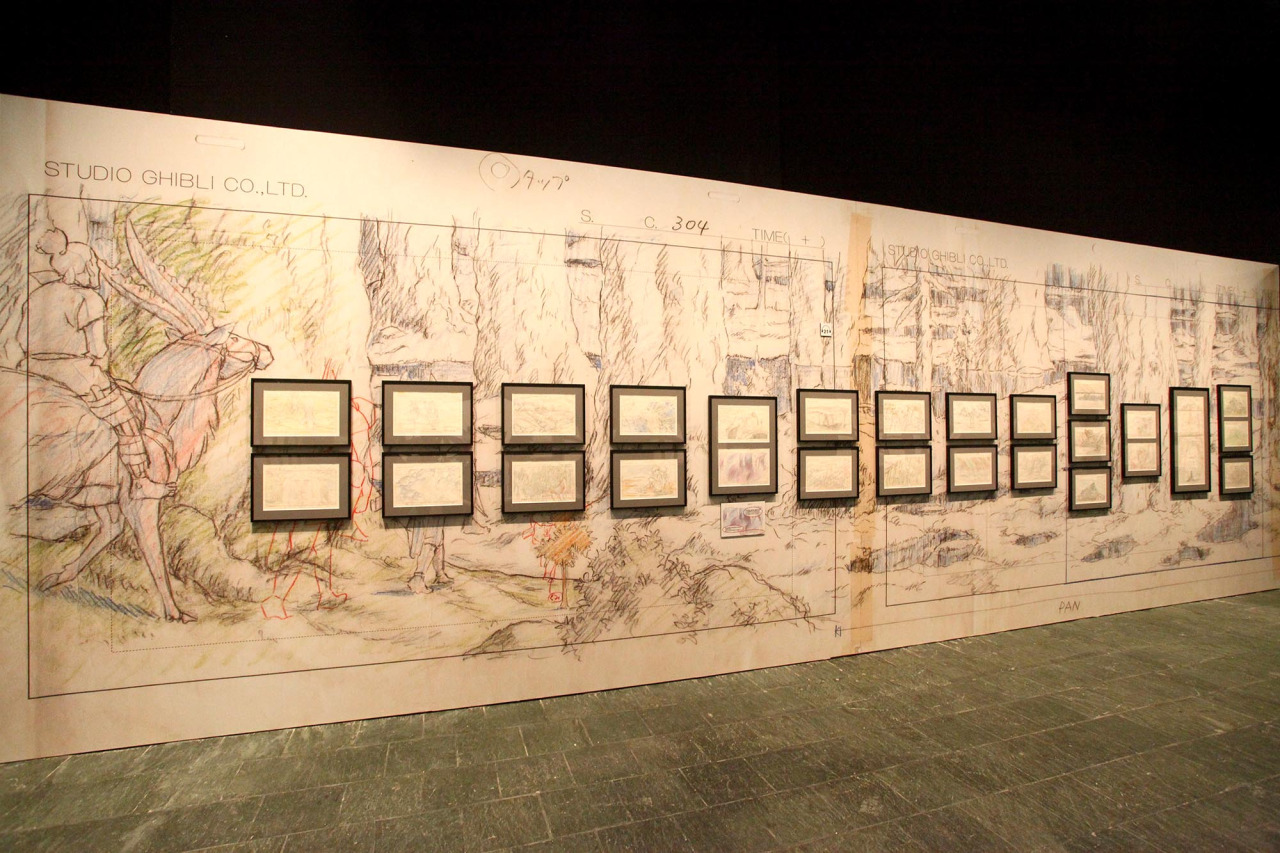
\includegraphics[width = 90mm]{PictureWall.jpg}
\caption{An exhibition piece used as background image at the Studio Ghibli Layout Designs exhibition in the Hong Kong Heritage Museum \cite{ghibli}}
\label{fig:picturewall} % deze regel niet naar boven verplaatsen, dan gaat referencen stuk.
\end{figure}

\item{\textbf{Picture in style of the painting}}
\\With the algorithm of Gatys et al.~\cite{gatys}, a picture is altered to look like it was painted in the style of a given painting. An image is produced that still shows the content of the picture, but it appears to be painted in the same style as the painting. Instead of using a regular picture as in the example above, the picture could be processed to get the same style as the painting. That picture can then be displayed on the wall behind the painting. This could make for a better backdrop to the painting than a regular picture would, as it resembles the painting more. Since the algorithm can be applied to any type of image, three different ways of applying it in our museum setting come to mind. 

Firstly, the style of the painting could simply be applied to a single object in the environment, such as a picture projected on a wall. This could easily be done in preprocessing. 

Secondly, the style could be applied as a post-processing effect to the user's field of view. Each frame the user sees through the VR device will be processed to have the same style as the painting. However, some issues can be foreseen with this type of application, as processing might take too long to maintain a decent framerate. Additionally, a very subtle change in head orientation could cause a very large change in the rendered view, as the entire frame would have to go through the stylization process again. 

Finally, we can apply the style of the painting to the textures of all objects in the room. This way we can take advantage of preprocessing and therefore avoid the drawbacks of the previous method. A possible downside is that the illusion would only be applied to textures, and therefore would not affect 3D shapes and shadows.

\item{\textbf{Extending the painting}}
\\If a painting is a window into the world of the painter, then what lies beyond that window? With a method called inpainting \cite{inpainting}, it is possible to extrapolate information from the painting and apply it to the empty wall surrounding it. In this way, the wall can be made to look like an extension of the painting - like the wall and the painting are actually one big painting.

\end{itemize}

\subsubsection{Animated Visual Illusions}\label{sec:animeffects}

Some illusions mentioned in the previous section can also have an animated variant, and some illusions can only be achieved when animated.

\begin{itemize}

\item{\textbf{Changing colors on the wall}}
\\In the virtual space, the wall would not need to be one color, but could change color over time to create different moods.

\item{\textbf{Video related to the painting}}
\\A video would be the more dynamic version of the still picture. For example, behind old news pictures, a news video covering the same event could be shown. The emphasis would still be on the pictures, and the video could intensify the experience by making the surroundings supplement the displayed art.

\item{\textbf{IllumiRoom 'weather illusions'}}
\\The idea of using images related to the painting can be extended to 3D. The room or the walls can be filled with particles that relate in some way to the painting, like snowflakes for a snowy painting or leaves for a painting of a forest in fall. Instead of basing these illusions solely on weather, they can be generalized to various particle effects based on the setting of the painting. These illusions are based on the IllumiRoom \emph{Snow} illusion \cite{illumiroom} and are discussed in more detail in section \ref{sec:methods}. %Is that indeed discussed in methods?

\item{\textbf{Picture in style of the painting}}
\\Another animated illusion uses a picture shown on the back wall, while the picture slowly morphs into the same style as the painting. In the algorithm of Gatys et al.\cite{gatys}, the grade of stylization can be controlled. In this way, multiple images can be produced that are in style somewhere in between the unaltered picture and the style of the painting. With those, an animation can be made of the picture slowly changing to match the style of the painting. Alternatively, interpolating between the normal picture and a fully stylized version without the intermediate steps is a cheaper method.

\item{\textbf{Extending the painting}}
\\For this animated illusion, the painting expands over the back wall while the user is watching it. This can be done by using painting expansion software \cite{inpainting}. The wall around the painting is filled with textures extrapolated from the painting.

\end{itemize}

\subsubsection{Auditory illusions} \label{sec:audioeffects}

Many different types of sound exist. This includes music, sound caused by something closeby, and ambient sound, the sound made by the environment. In our case, we aim to create a connection between the audio and the visuals of the painting. With this in mind, t ypes of audio can roughly be subdivided into two groups, audio related to the painting and audio related to the museum environment. A few examples of sounds that can be added to the experience will be given: 

\begin {itemize}

\item{\textbf{Music related to the painting}}
\\This can be music from the era of the depicted scene, or even music that could have been played by a person who is in the painting. It could also be modern music that is associated in some way to the subject of the painting. 

\item{\textbf{Music not related to the painting}}
\\A piece of music that is not deliberately chosen to match the painting, but, for example, chosen because it is favored by the people visiting a museum to view the paintings. This would add to the experience of visiting the museum, without the music having anything to do with the painting. 

\item{\textbf{Sound effects related to what is happening in the painting}}
\\An example of this is the sound of a hammer hammering metal for a painting of a smithy, or the sound of swords clashing or gunfire for a painting that depicts a war. 

\item{\textbf{Ambient sound related to what is happening in the painting}}
\\The sound of birds singing for a sunny painting of a landscape, the sound of rain and thunder for a painting of a thunderstorm or the sound of people talking and yelling for a painting depicting a market - these are just a few examples of ambient sound that you would hear if you were standing in the painting.

\item{\textbf{Ambient sound of a museum environment}}
\\This one is more like the music unrelated to the painting - it is also an example that focusses on the museum instead of the painting. It adds the sounds one would hear when visiting a museum: soft shuffling of feet, footsteps, murmuring or whispering of people talking about what they see. 

\end{itemize}

%Based on testing on a small scale, three types of audio were selected as being the most promising for our purposes. <-- deze hier onder toevoegen

\begin{itemize}

\item{\textbf{Ambient sound related to the museum}}
\\This type of audio consists of various noises that are commonly heard in museums. This includes footsteps, mumbling and other low volume noises. %The main goal for this type of audio was to replicate the sounds heard when visiting an museum and therefore increasing the user's sense of presence in the virtual museum. %This type of audio was played continuously on one floor for each participant, since interrupting it temporarily in the hallway would feel strange based on our experience, and wouldn't be consisting with the experience in an actual museum.

\item{\textbf{Ambient sound related to the painting}}
\\For this type of audio, ambient sound is selected based on the content of the painting. For example, a painting depicting a forest scene is accompanied by sounds of singing birds and wind blowing through leaves. %The main goal for this type of audio is to create connectedness with the painting it is related to. %Because the audio was based on the contents of a painting, it was only played in rooms containing paintings.

\item{\textbf{Music related to the painting}}
\\For this type of audio, music is selected based on the content of the painting. Since this is a highly subjective matter, we base our music on existing examples such as video games and movies. %This type of audio is meant to serve multiple purposes, both increasing the presence and connectedness. %Since it was related to the paingtings, the audio was only in rooms containing paintings.

\end{itemize}


\subsection{Utilized design space} \label{sec:utilized design space}

For this research, the animated illusions of the stylized picture, extension of the painting and the IllumiRoom weather illusion appear to be the most promising to see as a visual effect. These illusions can be applied to almost any kind of painting and use modifications based directly on the painting. They can be customized extensively to fit the need of the user or curator, but also leave open the option of automatization. As these illusions are animated, they are very hard or even impossible to create in real museums. However, by utilizing the aspects of virtual reality, these illusions can be created in a virtual museum.

Not every type of illusion is suitable to be applied on both the wall around the painting as well as in the 3D space. It makes sense that the stylized and extension illusions are applied on the wall as they are envisioned on a surface. The weather effects can also be applied on a wall, but we intend to utilize the possibilities of VR and create the weather illusions in 3D space. In Table \ref{tab:ourillusions}, the suitable combinations that are going to be tested can be found.

As for the auditory illusions, the three examples mentioned in \ref{sec:audioeffects} seem to be  promising choices. The different types of sounds can also be combined, but to keep this experiment as clean as possible, the different types of sounds will be separately played from each other. It makes sense to play museum ambient sounds during a whole museum visit, to create a feeling of a museum as a whole. As for the other two types, it is better to play them near a painting as the sounds are painting specific. There is a possibility to make use of 3D sound, that the sounds are coming from a certain direction. However, if the sounds are coming from a certain direction, it might influence the sense of direction of the user. This can conflict with the goal to create the feeling of being in a different environment. (The goals of the illusions will be discussed in the next section.) To avoid possible issues, the sounds will have no particular direction. %It make The audio will play in the whole room, and does not come from a particular direction. % possibly TODO, dunno of we er meer over willen zeggen. ALSO laatste zin 'will play' past dat wel?

\begin{table}
\centering
\begin{tabular}{l|cc|cc|}
\cline{2-5}
\textbf{} & \multicolumn{2}{c|}{\textbf{Space}} & \multicolumn{2}{c|}{\textbf{Animation}} \\ \cline{2-5} 
\textbf{} & \textbf{Wall space} & \textbf{3D space} & \textbf{Static} & \textbf{Animated} \\ \hline
\multicolumn{1}{|l|}{\textbf{Stylized}} & $\surd$ &  &  & $\surd$ \\ \cline{1-1}
\multicolumn{1}{|l|}{\textbf{Extended}} & $\surd$ &  &  & $\surd$ \\ \cline{1-1}
\multicolumn{1}{|l|}{\textbf{Weather}} &  & $\surd$ &  & $\surd$ \\ \hline
\end{tabular}
\caption{\label{tab:ourillusions}The illusions used in this research and their tested spaces in the room}
\end{table}

\subsection{Illusion goals}\label{sec:illusiongoals}
As we compare the effect and goals of each illusion, it seems that certain illusions are better suited to enhance a certain aspect of the user experience. The stylized and extending illusions are 2D effects while the weather effect is 3D. The 2D property of the stylized and extending illusions stay more true to the 2D nature of paintings and the original idea of the museum. For this reason, we will focus more on the enjoyment and interest in art and museums aspects of the experience with these illusions. 
The weather effect, however, creates this new 3D space filled with particles which is not usual in museums. Because of this new space, this type of illusion is more interesting in terms of presence. This also gives this type of illusion the opportunity to use sound as well, to increase the sense of presence and connectedness (presence in the world of the painting) even more. The museum ambient sound replicates the sounds heard when visiting an museum and therefore increasing the user's sense of presence in the virtual museum. The painting ambient sound and music are painting specific, and are thus better suited to create connectedness. 

To answer our research questions, we will split these goals up into two pilot studies:
\begin{itemize}
\item{Part 1:} Measuring enjoyment and interest in art and museums with the stylized and extending illusions.
\item{Part 2:} Measuring presence and connectedness with the weather illusions and sounds.
\end{itemize}
Even though the goals for each part are different, it does not mean that they are mutually exclusive. The goals indicate a focus on a certain aspect of user experience for a user study. Without this split, evaluating all the aspects in a single user study would be very difficult. Finally, the overall user experience will be evaluated.

\section{Methods} \label{sec:methods}

\subsection{Database}
%uitleg nodig dat 12 paintings voldoende is om te generaliseren?
To answer our research questions, we implemented various illusions for different paintings and use them to conduct a user study. Paintings with different three types of content, painted in two different artistic styles will be used. For each combination, two different paintings will be selected as a representation. Participants are allowed to participate in both part 1 and part 2. To prevent them from getting bored by seeing the same paintings we used two sets of paintings; set 1 in part 1 and set 2 in part 2. This means that we will use a total of 24 different paintings. In order to achieve reliable results, the paintings will be carefully selected, so that they provide a good representation of a large collection of paintings. The selected paintings for part 1 can be found in appendix~\ref{sec:paintings}. With this selection, we aim to provide a fair sample of a vast group of paintings they belong to.

For the content we will use the following categories:

\begin{itemize}
\item \textbf{Forests.} Paintings of forests, depicting trees and other foliage.
\item \textbf{Seascapes.} Paintings of open sea or seashores.
\item \textbf{Snowy environments.} Paintings of landscapes covered in snow and paintings where snow is falling.
\item \textbf{Rainy environments.} Paintings where it is raining in the scene.
\end{itemize}
We have chosen these categories because they are general enough to represent a large subgroup of all paintings, yet they are easy to distinguish between because of their well-defined characteristics. For part 1, forest, seascape and snowy environment paintings are used. For part 2, forest, snowy environment and rainy environment paintings are used.

We will use the following artistic styles:

\begin{itemize}
\item \textbf{Photorealistic paintings.} Paintings depicting the content in an accurate and realistic way.
\item \textbf{Stylized paintings.} Paintings depicting the content with a distinctive style, like coarse brush strokes.
\end{itemize}

We have chosen these two different styles to be able to investigate the effects of the illusions for different types of paintings. If an illusion works well for a photorealistic painting, it doesn't imply that it also works well for a stylized painting. Some of the illusions rely heavily on the style of the painting, meaning their impact could be different when combined with these two artistic styles.

As discussed in section \ref{sec:utilized design space}, we will apply the following three animated illusions for each painting in their corresponding set:

\begin{itemize}
\item \textbf{Stylized picture.} For this illusion we will overlay a picture on the wall behind the painting. The style of the painting will be applied to the picture using methods described by Gatys et al.\cite{gatys}. Pictures will be different for each painting and will be selected to have content similar to the painting. This illusion will be animated by interpolating between the original picture and the stylized picture.
\item \textbf{Inpainting.} For this illusion we will display and extend content based on the painting on the wall behind it using the inpainting algorithm \cite{inpainting}. In the final state of the animation, the extended image will cover the whole wall behind the painting. 
\item \textbf{Weather-like effects with sounds.} For this illusion we will create 3D particles based on the weather conditions and content of the painting. These particles will include snow, rain or falling leaves and fall in the 3D space of the room. Accompanying the weather-like effects, a type of music (museum ambient, painting ambient or music) will be played. 
\end{itemize}

\subsection{Hardware and Application}
The application is implemented using Google Cardboard. Google Cardboard is a VR device that uses a smartphone as a display. This device has the benefit of being cheap, portable and easy to use, making it easily accessible to museums or individuals. 

The HMD used for this experiment was the Hema VR glasses, a basic VR device that can be bought by a normal consumer. It has adjustable straps that attach the headset to a person's head. The lenses in the device can also be adjusted: both the distance between the lenses and the screen as well as the distance in between the lenses could be adjusted. A mobile device can be put in to serve as the display. 

The mobile device used for this test was a Sony Xperia Z5 Premium, a 5.5-inch screen with a resolution of 2160x3840 pixels. The application however, runs in 1080p on the device. As for sound, Sony DR-BTN200 wireless headphones were used. The headphones were wireless to avoid complications with the cables as the user has to look around and rotate in a rotating chair. (This setup will be explained in the next section.)

The application visualizes a virtual museum. This museum is not based on any existing museum and consists of different floor with rooms. The paintings can be found in the rooms and each room contains only one painting combined with a certain illusion to isolate the effect of it (Fig \ref{fig:stylizedExample}, Fig \ref{fig:extendedExample} and Fig \ref{fig:weatherExample}). The user can look around by moving his head and navigate trough the virtual space by only looking. To enter rooms or next floors, the user has to keep looking at a door. The doors function like a loading bar. When this bar has been loaded, the user will be teleported to the next location. The use of any control devices, such as gamepads, have been ommitted so that users do not have to pay attention to control such devices and can keep there focus in the application itself. It is also a way too restrict the users' movement to gain more control in what the users do, and most importantly to lower the chances of cyber sickness.

%controls, design decisions% 

\begin{figure}
\centering
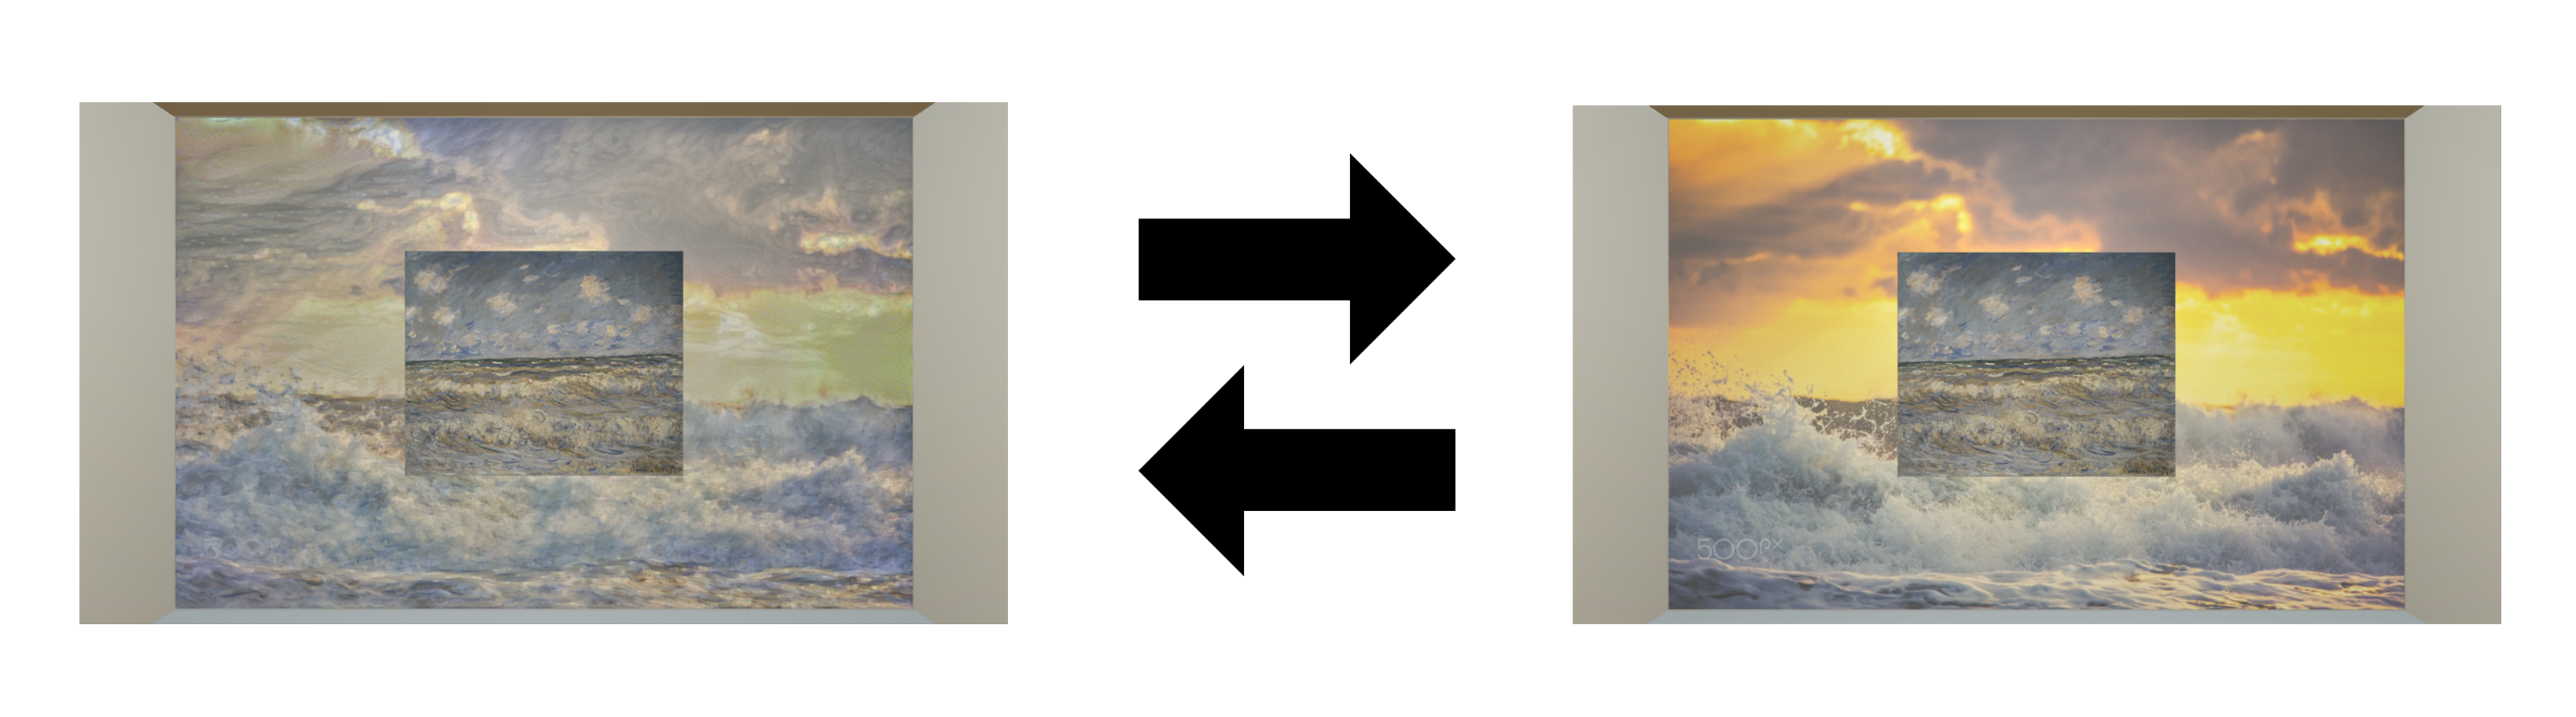
\includegraphics[width=12cm]{StylizedExample}
\caption{Stylized picture illusion. The image on the wall behind the painting interpolates automatically between the original picture and the stylized picture}
\label{fig:stylizedExample}

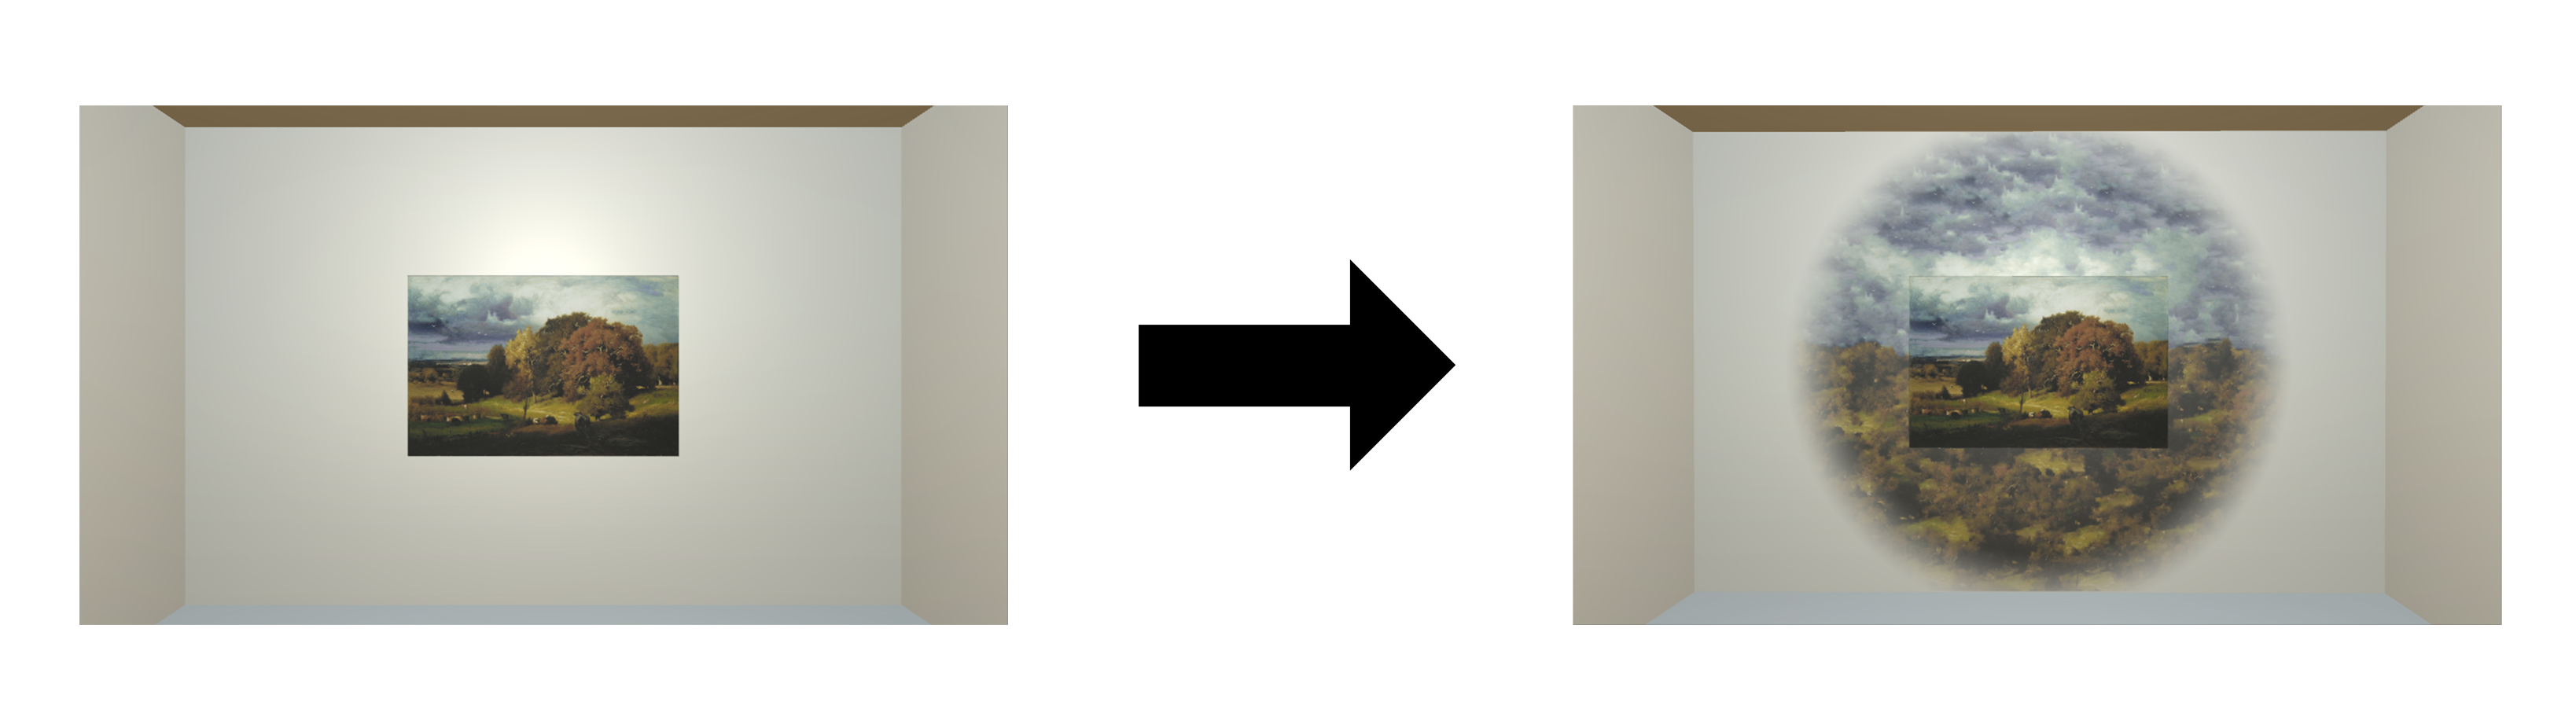
\includegraphics[width=12cm]{ExtendedExample}
\caption{Inpainting illusion. The image will be extended over the wall behind the painting at the moment the user enters the room. The animation can be triggered again by looking at a button near the feet.}
\label{fig:extendedExample}

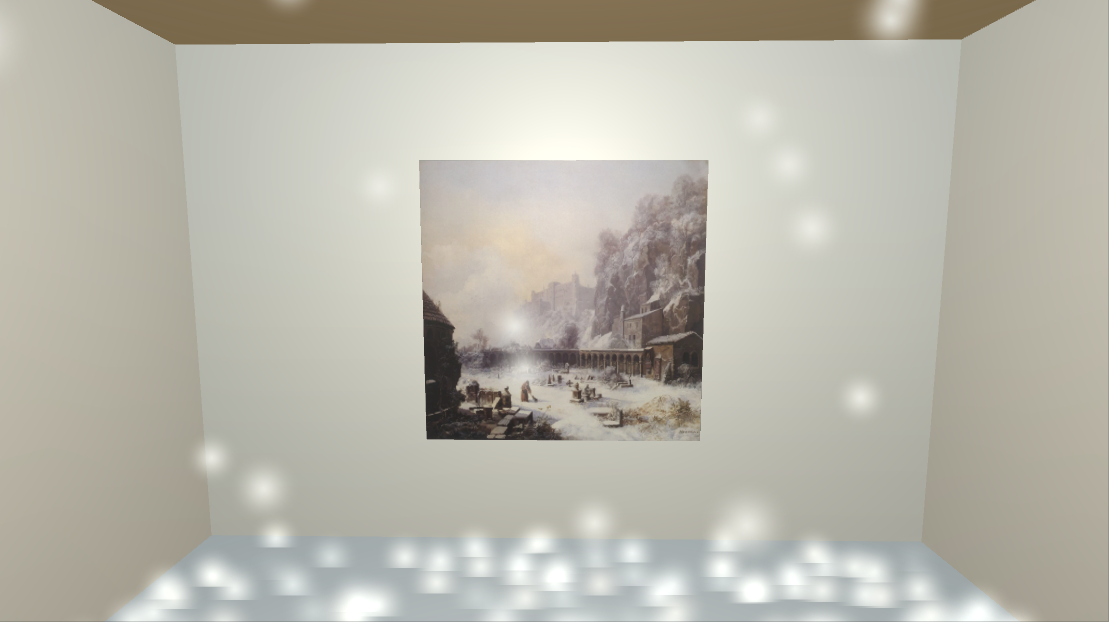
\includegraphics[width=5cm]{WeatherExample}
\caption{Snow weather illusion. Snow constantly falls down in the room with the painting.}
\label{fig:weatherExample}
\end{figure}

\subsection{Experiment Setup}

%The animated illusions can be implemented in various ways, including different values for parameters such as speed or behaviors of animation. To get a set value for these settings, a pre-experiment will be done to find the most promising settings in terms of enjoyment and presence. This can first be done internally and then tested on three to five people, giving their opinion about the different settings of the illusions. These participants are not allowed to join the main experiment anymore as they have seen the illusions before. This can influence their final judgment.

% ^ update v

The animated illusions can be implemented in various ways, including different values for parameters such as speed or behaviors of animation. To find good values for these settings with respect to our research goals, a small pre-experiment was conducted. For this pre-experiment, we tested the application ourselves and with a few other people who did not take part in the main experiment. The parameters were set based on the opinions gathered from these tests.

% Beschrijf parameters/illusies hier (incl. loop/replay button).

% For the main experiment, combinations of paintings and illusions will be subdivided into four groups. This is done to create four different combinations, where every painting-illusion combination can be rated by a user who has not seen that painting in our museum setting before. This means that each group will consist of twelve paintings. This means there are three paintings of each illusion, and three paintings without an illusion per group. For each participant, the environment for the twelve settings will be similar. Every time they will be placed in a room based on a part of a museum. The room will contain one painting and will have some additional objects such as chairs or plants. Apart from this, the room will be fairly plain in order to avoid distraction.

For both parts of the main experiment, different setups were used based on the required results. These setups are explained in Sections \ref{sec:setup1} and \ref{sec:setup2} for part 1 and part 2 respectively.

\subsubsection{Setup part 1}\label{sec:setup1}

% Setup experiment 1 hier, inclusief setup.txt uitleg, volgorde en questionnaires/interviews.
Part 1 of the experiment contained of a virtual museum setup consisting of four floors. The first floor was used as an introduction, while the remaining three floors formed the main part of the experiment. Each floor contained three doors leading to rooms with paintings in them. On each floor, one room contained no illusion, one room contained the inpainting illusion, and one door contained the stylized illusion (Fig \ref{fig:part1Layout}). On each door leading to a room with a painting, an icon was displayed, indicating the type of illusion in that room. These icons were shown to the participant on paper beforehand. Whenever the participant has entered a room, the corresponding door will be marked with a check mark to indicate which rooms have been entered before. 

\begin{enumerate}
\item The participant was asked to sign a consent form related to potential health risks of VR. This form also contained a small introduction about the experiment.
\item The participant was asked to fill out a small survey containing general questions about the participant, their experience with VR and their interest in art.
\item The participant was given a verbal introduction and instructions to the first test. After these instructions, the participant sat down in a rotatable office chair and put on the HMD.
\item The participant was guided through the first test. This test consisted of a single museum floor with three adjacent rooms. Each of these three rooms contained the same painting, which was Van Gogh's Starry Night. The participant was asked to enter the three rooms in a specific order, enforced by the application. Each participant would first enter the room without any illusion. Secondly, half the participants would enter the room with the inpainting illusion, while the other half would enter the room with the stylized illusion. Finally the participants would enter the only room they had not entered before. In each room, the participant was asked to stay as long as they liked. Afterwards, they could return to the hallway of the floor and go to the next floor using the elevator door. On this next floor, a message was displayed, asking the participant to take off their headset.
\item An interview was conducted, asking the participant about their opinion about the different rooms and their interest in art and VR museums after seeing the illusions.
\item The participant was given instructions for the second test. In this test, the participant explored the remaining three floors. The participant could enter the rooms in any order they preferred, but had to visit all rooms on a floor at least once before advancing to the next floor. The participant could not go back to a previously visited floor.
\item The participant was asked to fill out an enjoyment questionnaire. It consisted of five likert scale questions about how the participant felt during the experiment. The second part of the questionnaire consisted of likert scale questions where the participant had to rate each emotion for each type of illusion (including no illusion). The words describing the emotions were chosen similar to how the PANAS questionnaire~\cite{panas} was developed. Like with PANAS, words were taken from Zevon \& Tellegen \~cite{zevon}. However, some new words had to be used as most of these words did not make sense in a virtual setup. In our case, the positive words were \textit{enthusiastic}, \textit{at ease}, \textit{joyful} and \textit{amazed}, and the negative words were \textit{distressed}, \textit{bored}, \textit{irritated} and \textit{sleepy}. The positive and negative words were shuffled, but always shown in the same order.
\item Another interview similar to the first interview was conducted. The goal of this interview was to find out if opinions had changed after seeing a more elaborate setup, and to gather more opinions on the illusions and specific rooms.
\item A memory test was conducted to see how well the participant remembered certain paintings. The participant was not informed about this test beforehand.
\item The participant was asked for any further comments or questions and thanked for their participation.
\end{enumerate}

As discussed before, a total of twelve paintings were used for part 1. For each participant, nine of these twelve paintings were required due to the setup of the experiment. We created six different setups for the virtual museum. Doing so, we ensured that realistic and stylized paintings were both combined with each illusion the same amount of times, and that each type of content (forest, sea and snowy paintings) was combined with each illusion the same amount of times. Furthermore, paintings were distributed over the floors, such that no floor contained three paintings with the same type of content. Per participant, the order of the three types of rooms was different for each floor, such that each illusion was shown once behind each door.

\subsubsection{Setup part 2}\label{sec:setup2}

% Setup experiment 2 hier, inclusief setup.txt uitleg, volgorde en questionnaires/interviews.
Part 2 of the experiment contained a virtual museum setup consisting of five floors. The first two floors were part of the introduction. The third floor formed the main floor to test the sense of presence and connectedness of  the participant. This floor consisted of three rooms with a painting in each of them. The last two floors have the same layout as the third one, but deviated from the third floor in the used paintings and sound (Fig \ref{fig:part2Layout}). Each door leading to a room have an icon on them, indicating the weather effect in the room. After the participant has entered a room, the corresponding door to the room will also be marked with a check mark, just like in part 1.  

\begin{enumerate}
\item The participant was asked to sign a consent form related to potential health risks of VR. This form also contained a small introduction about the experiment.
\item The participant was asked to fill out a small survey containing general questions about him- or herself. It also contained questions about the participant's experience with VR and the interest in art.
\item The participant was given a verbal introduction and instructions to the first test. After these instruction, the participant sat down in a rotatable office chair and put on the HMD.
\item The participant was guided through the first test. This floor had a door leading to a room with a painting of Vermeer's Girl with a pearl earring. After viewing this painting the participant advanced to the next floor. This floor consisted of three doors leading to other rooms. Each room had a different weather effect and painting in them. The participants were asked to visit each room and to look at the paintings in any order and as long as they liked. After this, the participant entered the next floor, asking them to take off their HMD.
\item A short break was introduced. This break was meant to let the player slowly getting used to the VR view with short sessions to lower the chances of cyber sickness. During this break, short questions were asked about their general thoughts about the application. 
\item The participant was given instructions for the second test. They have to enter each room again on the new floor in any order they would like and look at the paintings as long as they wanted. The participant puts the HMD back on, this time including the headphone (Fig \ref{fig:part2Setup}), and takes the second test. After entering the next floor, the participant had to take off the HMD and headphone again.
\item The participant filled out a presence and connectedness questionnaire. The presence part of the questionnaire was based on Slater \& Steed's questionnaire~\cite{slater}, and the connectedness part was an altered version of it to accommodate for the extra dimension. %worldception
\item An interview was conducted with the participant. The interview contained questions asking what the participant liked and disliked about the different rooms and what their opinion was on the weather effects and the sound.
\item The participant was asked to put on the HMD and headphone again and start the third test. The participant has to visit all the rooms at least once in any order they like and look at the paintings as long as they want. However, the participant could not go back to a previously visited floors. 
\item The final interview asked the participant about their opinion on the last two floor he or she saw. It also asked about which floor(s), room(s) and sound(s) they like and disliked the most in the entire experience, and if some of them had a greater influence on their sense of presence or connectedness. 
\end{enumerate}

For part 2 of the experiment, twelve different paintings were used. Each painting was combined with a weather illusion which complements the theme of the painting. Also, each painting got combined with each type of sound. The type of sounds were different between the floors. The museum ambient sounds were played during the visit of a whole floor. The painting ambient and music were only played in the rooms of the painting. The order of the floors with sounds were shuffled in Latin square, this resulted in three different setups.

\begin{figure}
\centering
\captionbox{Example setup of part 1. Each cube depicts a room, and each color (red, green and blue) is a different type of illusion. \label{fig:part1Layout}}[.45\textwidth]{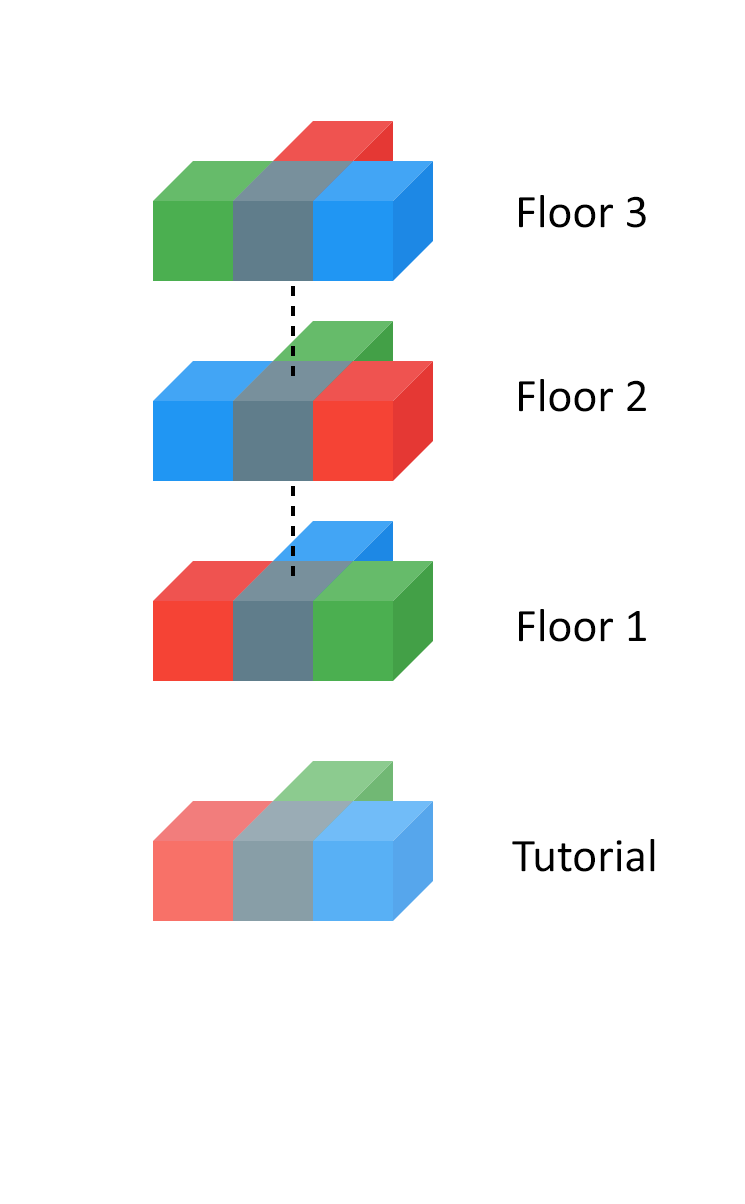
\includegraphics[width=0.45\textwidth]{Part1Layout}}
\hfill
\captionbox{Example setup of part 2. Each cube depicts a room, and each floor has a different type of sound. \label{fig:part2Layout}}[.45\textwidth]{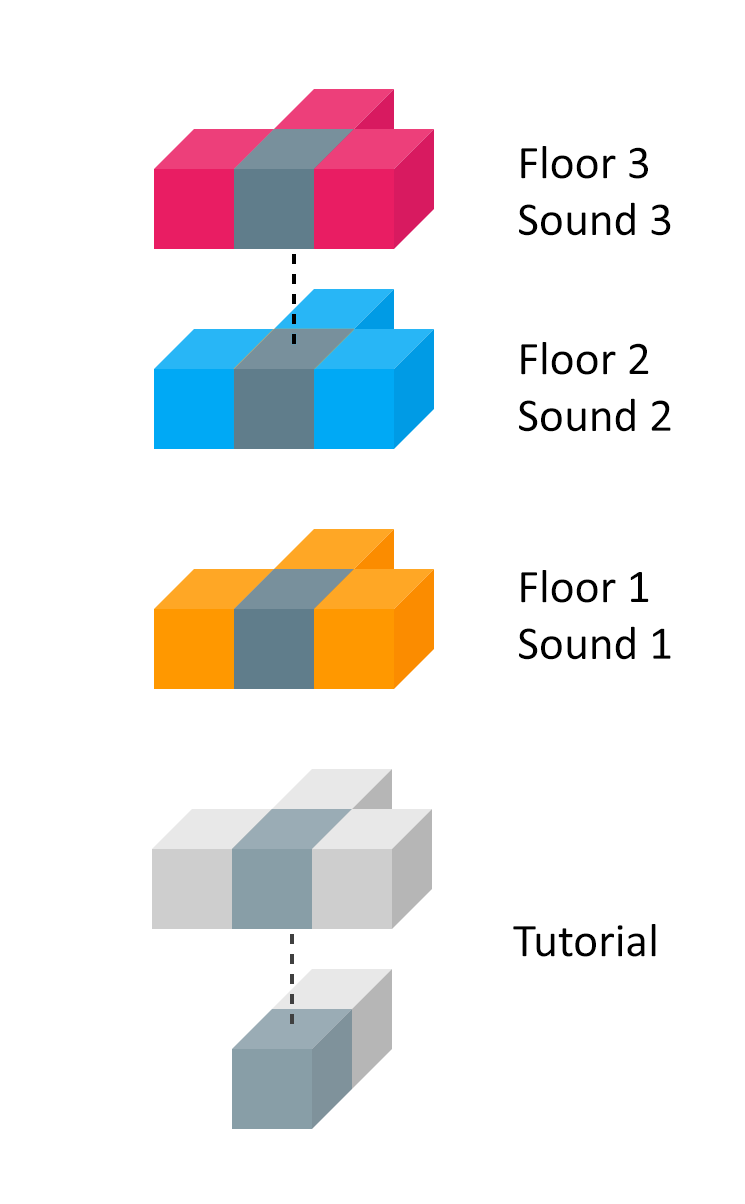
\includegraphics[width=.45\textwidth]{Part2Layout}}
\end{figure}

\begin{figure}
\centering
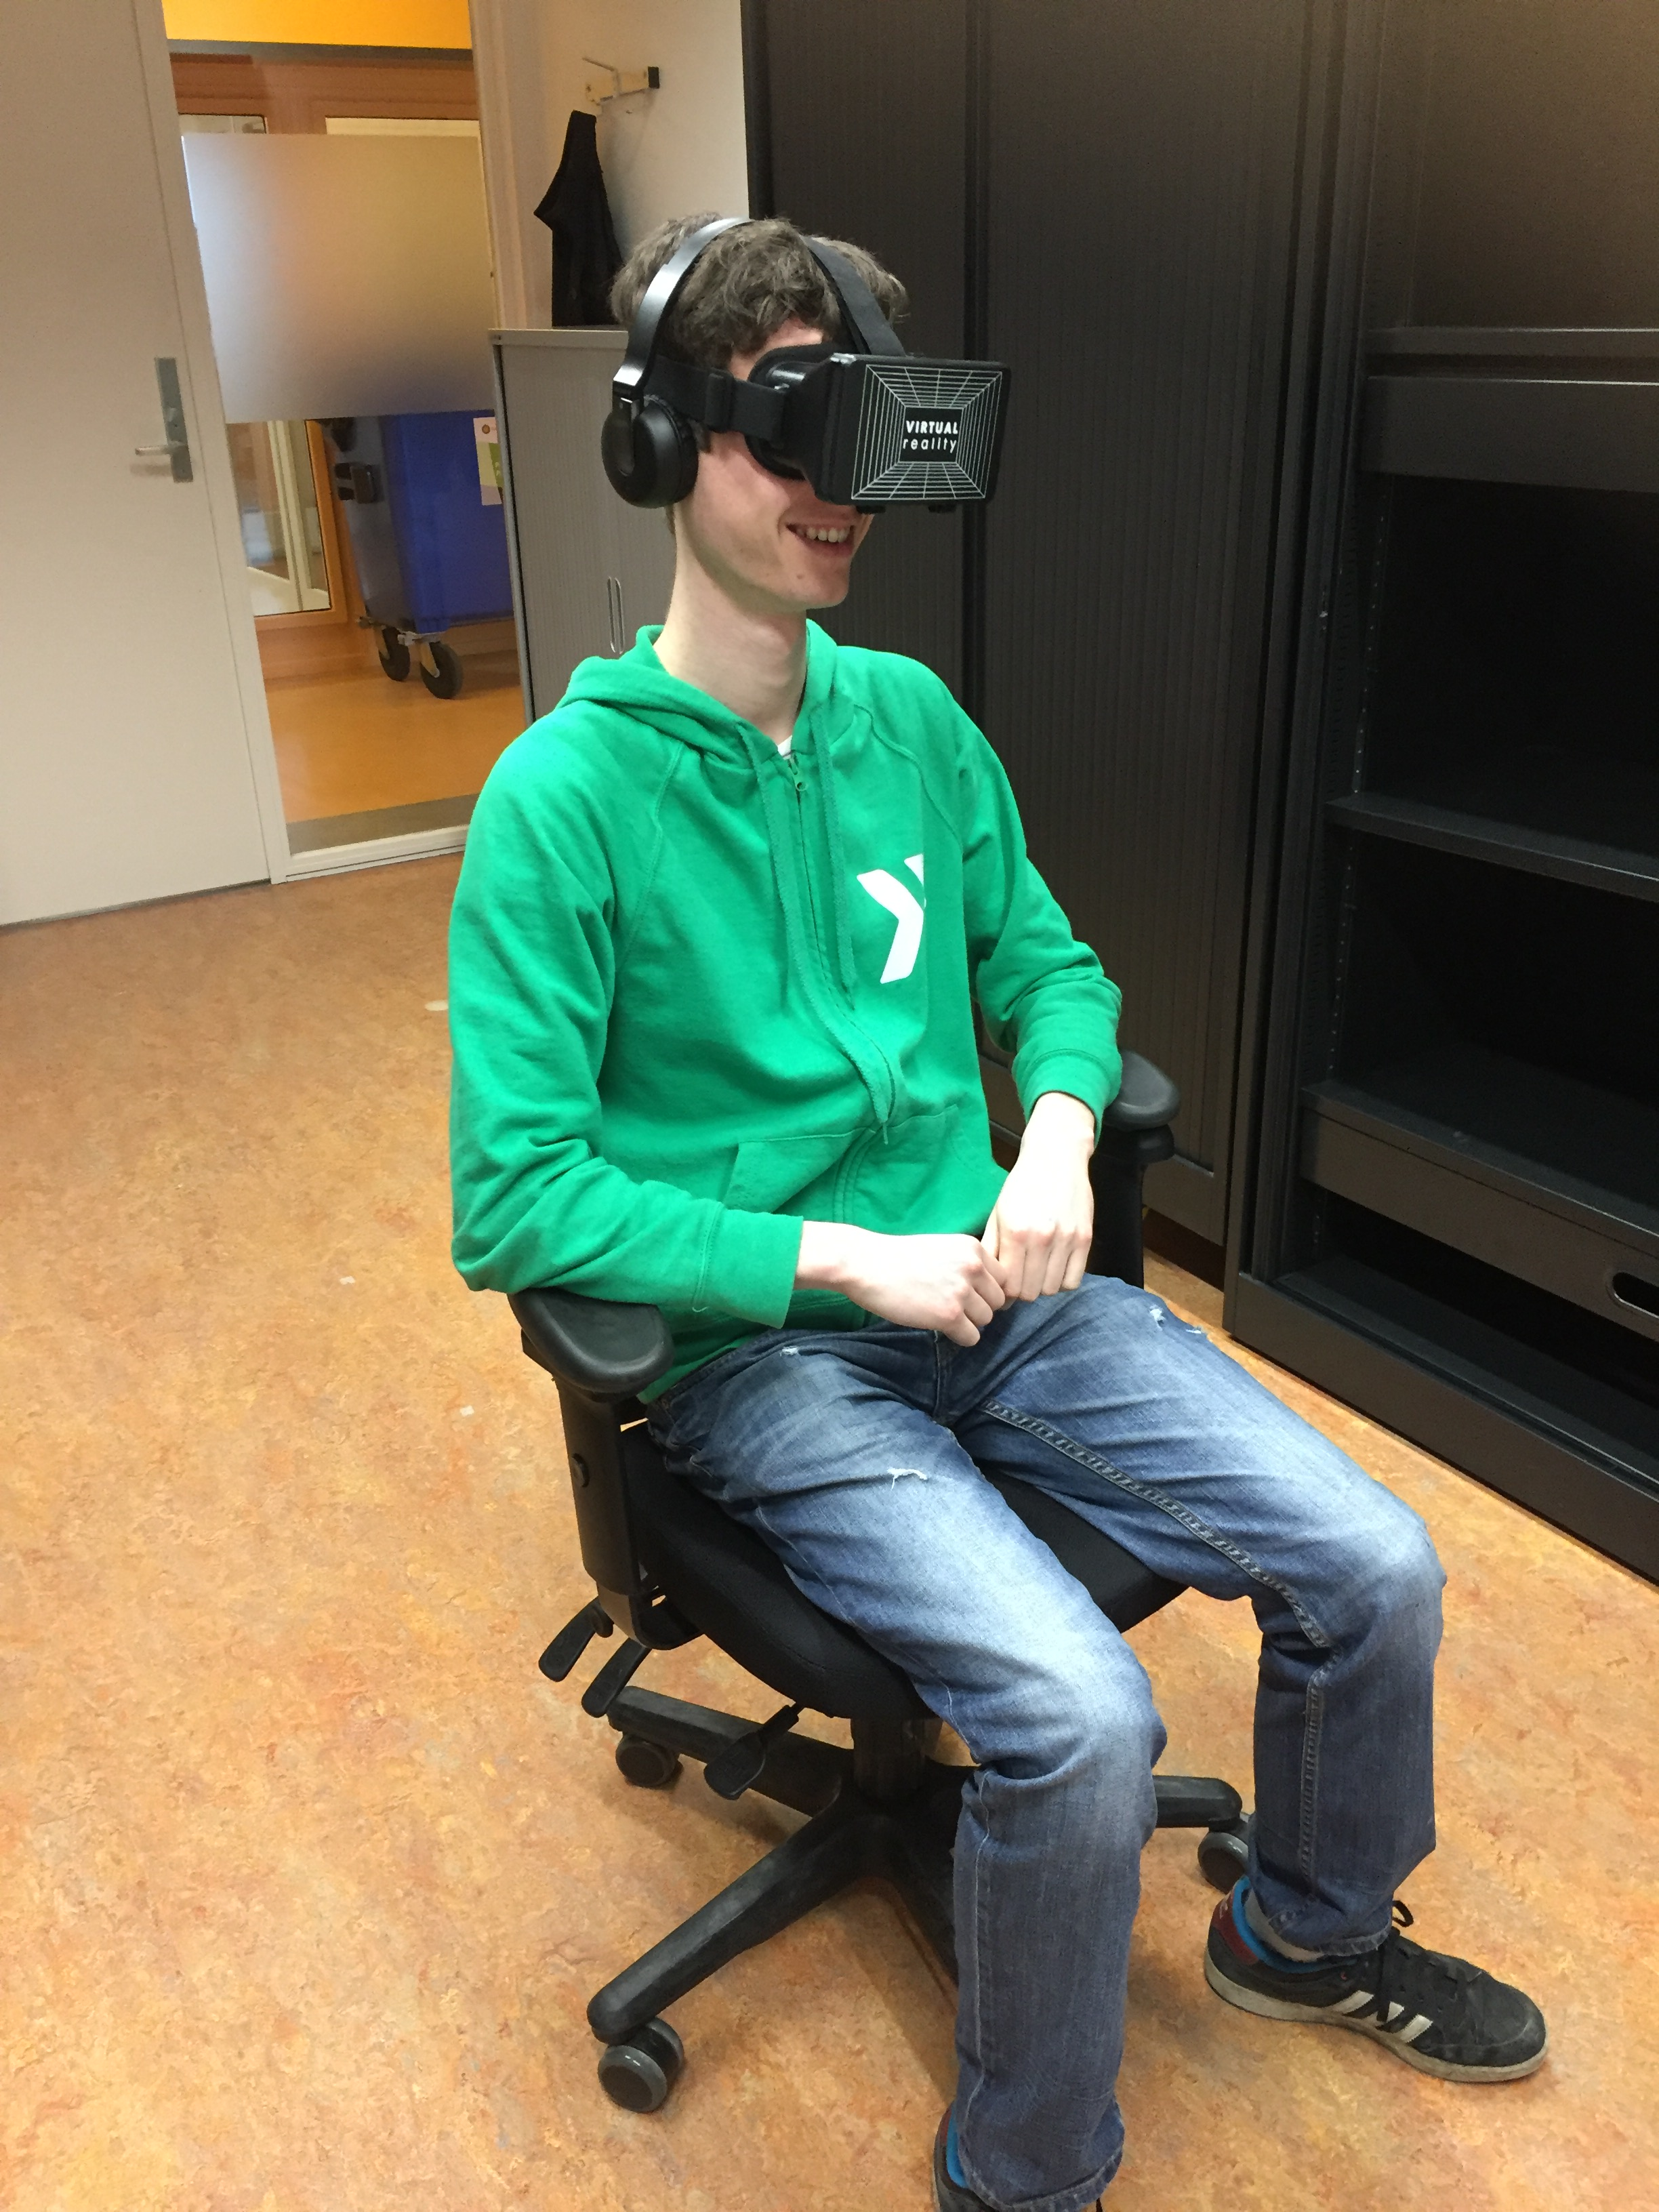
\includegraphics[width=7cm]{Part2Setup}
\caption{A user sitting in a rotating office chair with the HMD and headphones.}
\label{fig:part2Setup}
\end{figure}

% Deze section weghalen en per experiment uitleggen hierboven.
%\subsubsection{Measurements}\label{sec:measurements}

%The user will first be interviewed about their interest in art and willingness to visit art museums by means of a questionnaire. This questionnaire will then be repeated after the experiment so see whether their opinion has changed.

%Using a questionnaire, we capture the user's sense of presence in the virtual museum, connectedness (presence in the world of the painting) and enjoyment. This survey will be an adapted version of the presence questionnaire by Witmer \& Singer \cite{witmer}. We will have to come up with additional questions for the very specific subject of connectedness.

%To measure the participants' interest in the painting and the illusion, the direction in which they are looking will be tracked during the experiment. The amount of time the participants are looking directly at the painting or at the illusion will be measured in order to determine whether or not the environment draws away the user's attention from the painting. 

%The measured variables will be statistically analyzed. We will compare the results of all groups to determine the difference between each illusion and the default case. Our results will show the differences in terms of interest, presence and enjoyment for each combination of groups. These results will grant insight into the impact of the different illusions.


\section{Results}

In this section we will discuss the results of both parts of the experiment. % ###

\subsection{Part 1}

\begin{figure}
\centering
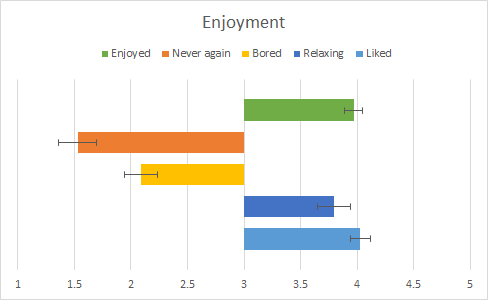
\includegraphics[width=8cm]{ResultsEnjoyment}
\caption{The average scores and standard errors of the enjoyment questionnaire.}
\label{fig:ResultsEnjoyment}
\end{figure}

\begin{table}[]
\centering
\begin{tabular}{|l|ccc|}
\cline{1-4}
\textbf{Word} & \textbf{None} & \textbf{Inpainting} & \textbf{Stylized} \\ \hline
\cline{1-4}
\textbf{Amazed}       & 1.9 & 3.7 & 3.4 \\
\textbf{Joyful}       & 2.5 & 3.3 & 3.2 \\
\textbf{At ease}      & 3.8 & 3.8 & 3.4 \\
\textbf{Enthusiastic} & 2.0 & 3.7 & 3.3 \\
\textbf{Sleepy}       & 1.8 & 1.5 & 1.5 \\
\textbf{Irritated}    & 1.4 & 1.3 & 1.6 \\
\textbf{Bored}        & 2.9 & 1.6 & 1.6 \\
\textbf{Distressed}   & 1.4 & 1.5 & 1.7 \\
\hline
\end{tabular}
\caption{\label{tab:panas}The results of the PANAS-style questionnaire.}
\label{t:panas}
\end{table}

The results of part 1 were obtained from the general questionnaire, the enjoyment questionnaire, the PANAS-style questionnaire, the interviews and the memory test. We will discuss these results in order.

\subsubsection{General Questionnaire}
There were 34 participants for part 1 of the experiment. The participants were all students participating in a computer science program at Utrecht University. From the general questionnaire, we obtained information about the demographics of our participants. The participants were between 20 and 29 years old, with the average age being 23. 76\% of the participants was male and 24\% was female. Participants generally indicated they were not that interested in museums, art or paintings. On average the participants visited a museum 0.9 times in the past year. Their interest in paintings and art was rated 2.8 and 2.5 on average respectively on a five-point Likert scale. Most participants had little experience with VR, mostly consisting of using a HMD once or twice. Two participants indicated they had previous experience with VR museums.

\subsubsection{Enjoyment Questionnaire}
The enjoyment questionnaire showed positive results. The enjoyment questionnaire consisted of five statements. Basing on their experience of the whole application, the participant had to rate them on a Likert scale from 1 to 5. In this case, 1 meant "completely disagree" and 5 meant "completely agree". The statements were as follows:

\begin{enumerate}
\item I liked the experience
\item The experience was relaxing
\item I was bored during the experience
\item I don't want to experience this ever again
\item I enjoyed the experience
\end{enumerate}

Statement 1, 2 and 5 were positive statement. Rating these statements higher means a more positive experience in terms of enjoyment. Statement 3 and 4 were negative statement. A higher rating of these statement indicates a not enjoyable experience. As shown in Figure \ref{fig:ResultsEnjoyment}, participants generally gave low scores to negative sentences and high scores on positive ones in the enjoyment questionnaire. 

\subsubsection{PANAS-style Questionnaire}
The averages for all the words per room type are shown in Table \ref{t:panas}. The scores were accumulated for the all the positive words. This was also done with the scores of the negative words. The results of the PANAS-style questionnaire also showed positive results and was heavily favored the illusions over the basic room, while slightly favoring the inpainting illusion over the stylized illusion. 
%For the positive words \textit{enthusiastic}, \textit{joyful} and \textit{amazed} both illusions scored significantly higher than the basic room, while for \textit{at ease} the stylized illusion scored significantly lower than both other cases. For  \textit{enthusiastic}, the inpainting illusion also scored significantly higher than the stylized picture illusion. For the negative words \textit{bored} and \textit{sleepy} both illusions scored significantly higher than the basic room. There were no other significant results.

\subsubsection{Interviews}
The participants were generally positive about the effects. When asked which effect the participants like most, the majority opted for the extending illusion. There were, however, some complaints about the illusions, like that they did not complement the paintings well enough, up to a point where they even get distracting. On the other hand, some said the contrary and praised that they fit very well. This issue is very hard, if not impossible, to solve as each person has his own opinion about art. It does mean that creating these illusions must be done carefully to please as many people as possible.

Comparing the rooms with illusions and the room without illusions during the second interview, no participant mentioned that he likes rooms without illusions the best. In fact, the room without illusions was rated the least liked room by 25 out of 34 participants. Some of the participants even mentioned that there would be no point in VR without the effects and that the art then can also be viewed on a computer screen. An interesting point about this remark is that the illusions were displayed on a flat surface (the back wall) and thus can also be visualized on a computer screen. Yet a few participants mentioned they felt more immersed with the illusions. In part 1 of the experiment we did  not look at the level of presence, but the relation between presence and these types of illusions might be interesting to look at in future work.

One participant, who said she has interest in art, particularly mentioned that seeing this application sparked more interest in art and VR museums. Generally, the effects encouraged people to visit VR museums if they have the chance and if it is free. A few of them even said that they are more likely to visit a real museum if they included illusions like these. Another participant thought that art should evolve into something like this and that if the artist knows what VR can do for him, the artist can base his art on that. Others also mentioned the benefit of VR museums for not having to physically go to a museum to enjoy art, however they also agreed that it would not be fully the same as in a real museum. In the end, these illusions are preferred in a VR museum for those who want something else than the standard museums, while those who do not wish for these artificial enhancements can enjoy the original artwork in real museums. 
  


\subsubsection{Memory Test}
The experiment concluded with a memory test. The participant was shown six sets of paintings, each of the sets consisted of four paintings. The participant had to mark the paintings they believed to have seen in the VR museum. Each set could contain none, one or two paintings the participant could have seen. The participants were told they could mark any number of paintings per set. The data was analyzed on correct answers, missed answers and false positives (paintings that the participant did not see but marked as seen). Through this data no trend could be found. An interpretation of these results could be that the illusions did not have a significantly distracting effect compared to no effect at all. It must be mentioned that this memory test was not based on a formal procedure, and that further research is required to confirm this initial conclusion.

% TODO: Interviews and memory test.

\subsection{Part 2}

The results of part 2 were obtained from the general questionnaire, the presence and connectedness questionnaire and the interviews. Again, we will provide an overview of these results below.

\subsubsection{General Questionnaire}
The demographics for this part of the experiment were similar to those of the first part. There were 25 participants aged between 20 and 26 years old, with the average age being 23. 72\% of the participants was male and 28\% was female. Experience with VR among participants was marginally higher than the first experiment, likely because some participants (10 out of 25) also participated in the first experiment. For the same reason, experience with VR museum apps was much higher, with 11 out of 25 participants indicating they had experience in this area.

\subsubsection{Presence and Connectedness Questionnaire}
The results from the presence and connectedness questionnaire were analyzed using one-way ANOVA ($\alpha=0.05$). For the presence part, the average of the scores of six 7-point Likert scale questions was calculated for each participant. This average was used as a score for their level of presence. Since each participant only answered the questionnaire for one setting (painting ambience, music and museum ambience). Although the music scored the highest in terms of presence (4.00 out of 7 on average), no significant results were found. Painting ambience and museum ambience scored 3.57 and 3.43 on average respectively. The results for connectedness were based on three 7-point Likert scale questions and analyzed in the same way. Again, no significant results were found. On average, music again had the highest score with 2.96, while painting ambience had a score of 2.22 and museum ambience a score of 1.75.

\subsubsection{Interviews}
The interviews that were conducted granted more insight into the sense of presence and connectedness of the participants and their opinions. Overall, participants were positive about the added weather effects and sound. Of the different sounds, music was preferred the most, with 16 participants stating music was their favorite type of sound. Additionally, multiple participants mentioned that music added to the sense of presence or immersion. The painting ambience was also perceived as positive in most cases. For this type of sound, participants emphasized the painting and connectedness over presence in the virtual museum. Museum ambience on the other hand was often viewed as negative or neutral. Most mentioned that the museum sounds did not match the actual virtual museum, since the sounds also contained footsteps and people talking even though the museum was empty. This created a mismatch between sound and visuals. Of the weather effects, preference was not as clear. The snow effect seemed to be the favorite. 10 participants preferring this effect over the other two, while 8 thought this was the worst effect. For rain, 6 people liked it best, while 10 people liked it least. For leaves, 6 people liked it best, while 3 people liked it least. It was interesting to note that some people mentioned that the weather effects influence their emotion or made them feel the weather. For example, one participant mentioned that he felt cold in the snow room, while another felt less at ease in the room with rain. These emotions were also sometimes influenced by the sound. Notable factors that influenced opinions about the weather effects were (in order of amount of times mentioned): the weather type, the level of realism of the effect, the particle size and the amount of distraction caused by the effect. The most mentioned factors related to presence were, in order: the sound, the weather, the complete view (due to VR and the 
ing chair) and the interactions with doors. Some people also mentioned that their presence increased over time and that it might be better to increase the duration of the individual tests. During the interviews, it became very clear that the exact choice and implementation of sound and visuals was very important. Every participant made comments about very specific things they liked or disliked. Examples include the music in a certain room not matching the painting, the sound being too loud or too soft, rain particles tilting when tilting your head or snowflakes staying on the floor after falling down. Finally, there were some other generally interesting comments. Firstly, the museum environment was important to participants. They especially liked the added plants and benches (which were not present in part 1). The environment influenced their enjoyment and presence in some cases. Secondly, some mentioned that it could be a good idea to combine multiple types of audio. For example, having museum ambience throughout the experiment, while adding music when entering a room with a painting. Finally, some people disliked the size and resolution of the painting, saying that they would like to be able to see more detail. This was sometimes mentioned as a factor in their connectedness to the painting.

\section{Discussion}

In this section we will reflect upon our research questions and answer them based on the results from our experiments. We will discuss the results as outlined in the previous section.

\begin{itemize}
\item Q1: \emph{How do illusions affect the enjoyment of viewing a painting in a VR museum setting?}

Our answer to this question is based on the PANAS and enjoyment questionnaires from part 1 of the experiment and the interviews from both parts. Based on these results, we can quite confidently say that the illusions had a positive effect on enjoyment. Only a few times the illusions were described as having a negative effect on enjoyment. Overall, every participant found that the illusions added to the enjoyment.

\item Q2a: \emph{How do illusions influence the sense of presence in the world of the virtual museum?}

Our answer to this question is based upon the presence questionnaire and the interviews from part 2 of the experiment. The presence questionnaire showed no significant differences. A possible reason for this is that the group sizes were quite low, with eight or nine participants per group. Significance could potentially be found by increasing the number of participants. Overall, music scored the highest in terms of presence. This was backed up in the interviews. This leads us to believe that out of the three types of sound, music has the most positive effect on the sense of presence. However, this is mostly based on subjective data. In general, sound seemed to increase the sense of presence, as long as it matched the expectations of the participants. Often, this wasn't the case with the museum ambience. The influence of different weather effects was not very clear. A number of participants mentioned that the weather had a positive effect on their sense of presence, but between the three types of weather there was no clear preference. Some participants also mentioned that the weather had a negative effect on their sense of presence because it felt strange to have these effects indoors. It seems that sound and weather effects can have a positive effect on the sense of presence when implemented well.

\item Q2b: \emph{How do illusions influence the sense of connectedness to the painting?}

Our answer to this question is based on the connectedness questionnaire and the interviews from part 2 of the experiment. The results mostly coincide with the results for the previous question. No significant results were found from the connectedness questionnaire. Music scored the highest, while museum ambience scored the lowest. Based on these results and the interviews, the answer to this question is the same as the answer to the previous question. It seemed the sound and weather had a positive effect on connectedness in most cases, while sometimes participants indicated that the effect was negative. This is again evidence for the statement that the specific choice and implementation of illusions is very important.

\item Q3a: \emph{How do illusions influence the interest in art?}

Based on our data, we can not conclude that the illusions influenced the interest in art of participants. In the general questionnaire at the start of the first user study, the average likert-scale score for interest in art was 2.8, on a scale from 1 to 5. In the final interview we added the question 'Do you have a different view about art now?' in order to discuss the participant's interest in art with them. Responses to this question were not in accordance with our expectations. Almost all of the participants simply answered 'No', and many indicated that the question was hard to understand. Therefore, we can not conclude whether or not the illusions influenced the interest in art of participants.

\item Q3b: \emph{How do illusions influence the interest in museums?}

Of the 34 participants for the first user study, sixteen had visited a museum over the past year. Thirteen of those indicated they would definitely visit museums more often if they would introduce illusions like the ones we added. Two of them included the condition that the application would have to be better than the one we showed them in a certain way. Most of these conditions were being able to move more freely. Fourteen out of eighteen participants who had not visited a museum indicated they would like to visit a real museum that displays these illusions after using our VR museum application. Eight of those, however, included similar conditions. In total, 27 of our 34 participants indicated they might visit a real museum or visit more often if the museum introduced illusions like ours, of whom 10 mentioned additional conditions. These results indicate a slight increase in interest in museums, although in some cases certain requirements would have to be met.

\end{itemize}


\section{Future research}

Based on our results, we would conclude that there are definitely a lot of interesting topics related to virtual museums to be explored further. Maybe the most obvious next step would be to increase the scale of the experiments to include more participants, paintings and illusions. This would make it easier to obtain quantitative data and find significant results that are more generalizable. Conversely, reducing the number of illusions to only one, and then testing this illusion with different parameters, could provide great insights as well and could lead to results that are easily applicable in practice.

There are also many options in terms of the implementation. First of all, different settings could be tested, as opposed to using a relatively plain museum setup. Some of our results, particularly interviews and open questions, suggested that this could create a lot of added value. For example, a painting could be displayed in an outside environments related to it. This could make the addition of weather effects seem more natural.

Related to the previous point, various mediums could also be tested. Using Augmented Reality or projectors in actual museums could create a completely different experience than when using VR. Each of these media has their own advantages and limitations, and exploring various options could lead to different and interesting results.

To more closely examine the interest in art or museums of participants, long-term research is essential. The behaviour of participants, including for example the amount of times they visit museums, could be monitored periodically over an extended period of time. Then, potential behavioral changes caused by using the app could be spotted, leading to more tangible results related to interest.

Finally, creativity appears to be very important in the domain of virtual museums. In this field of research, various disciplines can be combined. It appears to be of great value to work together with artists, designers and psychologists. Leveraging the expertise of these different disciplines could generate new insights and lead to more results.


%\subsubsection{Feasibility}
%The three illusions and the control without illusion serve as a 4-level categorical independent variable. With forty participants, this means that each illusion has been seen and rated 120 times, three times by each participant. Every unique painting-illusion combination will be seen and rated ten times. The central limit theorem can be used to prove a normal distribution in sample size of thirty or more. Forty participants seems more than sufficient. However, in ANOVA, the score has to have a normal distribution. Whether this is the case will have to be tested when the results are in. If a normal distribution cannot be proven, the Friedman analysis of variance by rank will have to be used. 

%Another issue is whether showing every painting-illusion combination ten times is enough. Since this research is about applying illusions to any painting, this is not an issue: each illusion is shown 120 times, to forty different participants.

%\section {Hypothesis \& Conclusion}
%We expect that every illusion will captivate users more than a regular painting in a white room would, causing them to use the application for a longer period of time. Adding these illusions will create a new virtual museum experience, that might pique the curiosity of those who are normally not interested in museums. They might take the virtual museum tour for the illusions, and will then be exposed to the paintings nevertheless, providing a chance to raise their interest in art. 

%This research will help expand the world of digital museums. In virtual reality, not everything has to behave like it would in the real world. This research explores and tries to expand the borders of virtual museums by adding illusions that would be impractical without the use of VR. This specific area is largely unexplored. Research in this area could open up a lot of possibilities.

%Real life museums could make their exhibits more interesting to people who would normally not visit them. This research could tell them what kind of illusion would be interesting to those people. These people could then look at the paintings through an Augmented Reality headset, or through the camera of their smartphone, while the regular visitors can still enjoy the painting on the background of a bland wall. Alternatively, they could visit parts of the museum in VR, and visit the real museum afterwards.



\begin{thebibliography}{99}

\bibitem{merriam} Merriam-Webster:
\emph{Dictionary}
Web [Last accessed on October 19, 2015]
http://www.merriam-webster.com/dictionary/virtual\%20reality

\bibitem{martens} Jon Martens \& Pavlo D. Antonenko:
\emph{Narrowing gender-based performance gaps in virtual environment navigation},
Computers in Human Behavior 28, p 809-819, 2012

\bibitem{kickstarter}
\emph{Oculus Rift: Step Into the Game}
Web [Last accessed on November 5, 2015]
https://www.kickstarter.com/projects/1523379957/oculus-rift-step-into-the-game/description

\bibitem{oculus}
\emph{Rift}
Web [Last accessed on October 20, 2015]
https://www.oculus.com/ja/rift/

\bibitem{gearvr}
\emph{Samsung Gear VR}
Web [Last accessed on October 20, 2015]
http://www.samsung.com/global/microsite/gearvr/index.html


\bibitem{tate1}
\emph{IK Prize 2015: Tate Sensorium}
Web [Last accessed on November 5, 2015]
http://www.tate.org.uk/whats-on/tate-britain/display/ik-prize-2015-tate-sensorium

\bibitem{tate2}
\emph{Welcome to Tate Sensorium: taste, touch and smell art - video}, 
The Guardian,  25 August 2015.
Web [Last accessed on November 5, 2015]
http://www.theguardian.com/artanddesign/video/2015/aug/25/welcome-tate-sensorium-taste-touch-smell-art-video


\bibitem{cardboard}
\emph{Google Cardboard}
Web [Last accessed on October 20, 2015]
https://www.google.com/get/cardboard/

\bibitem{wojciechowski} Rafal Wojcieshowksi, Krzysztof Walczak, Martin White \& Wojcieh Cellary
\emph{Building Virtual and Augmented Reality museum exhibitions},
The Poznan University of Economics, Poland,
University of Sussex, UK, 2014

\bibitem{westfries}
\emph{Kaap Varen}
Web [Last accessed on October 19, 2015]
http://wfm.nl/kaap-varen/

\bibitem{louvre}
\emph{Online Tours}
Web [Last accessed on October 19, 2015]
http://www.louvre.fr/en/visites-en-ligne

\bibitem{gatys} Leon A. Gatys, Alexander S. Ecker \& Matthias Bethge:
\emph{A Neural Algorithm of Artistic Style},
CoRR, 2015

\bibitem{witmer} Bob G. Witmer \& Michael J. Singer:
\emph{Measuring Presence in Virtual Environments: A Presence Questionnaire},
U.S. Army Research Institute for the Behavioral and Social Sciences, 1994

\bibitem{stevens} Stevens et. al.:
\emph{The Groningen Enjoyment Questionnaire: A measure of enjoyment in leisure-time physical activity},
Perceptual and Motor Skills, 2000

\bibitem{panas} David Watson, Lee A. Clark \& Auke Tellegen:
\emph{Development and validation of brief measures of positive and negative affect: The PANAS scales},
Journal of Personality and Social Psychology 54, p 1063-1070, 1988

\bibitem{zevon} Michael A. Zevon \& Auke Tellegen:
\emph{The structure of mood change: An idiographic/nomothetic analysis},
Journal of Personality and Social Psychology 43, p 111-122, 1982

\bibitem{illumiroom} Brett R. Jones, Hrvoje Benko, Eyal Ofek, Andrew D. Wilson:
\emph{IllumiRoom: Peripheral Projected Illusions for
Interactive Experiences},
Proceedings of the SIGCHI Conference on Human Factors in Computing Systems, p 869-878, 2013

\bibitem{inpainting}
\emph{Extending Van Gogh’s \emph{Starry Night} with Inpainting}
Web [Last accessed on October 19, 2015]
http://blog.wolfram.com/2014/12/01/extending-van-goghs-starry-night-with-inpainting/

\bibitem{slater} Mel Slater \& Anthony Steed:
\emph{The Influence of Body Movement on Subjective Presence in Virtual Environments},
Human Factors, 469-77, 1998

\bibitem{sylaiou} Sylaiou et. al.:
\emph{Exploring the relationship between presence and enjoyment in a virtual museum},
Int. J. Human-Computer Studies 68, 2010, pp. 243--253

\bibitem{mood}
\emph{Colour Theraphy}, 
The Guardian, 6 July 2008.
Web [Last accessed on November 5, 2015]
http://www.theguardian.com/lifeandstyle/2008/jul/06/healthandwellbeing.relaxation31

\bibitem{colorwall} Jonathan Jones
\emph{What colour should gallery walls be?}
The Guardian, 21 October 2011.
Web [Last accessed on November 11, 2015]
http://www.theguardian.com/artanddesign/jonathanjonesblog/2011/oct/21/colour-gallery-walls-musee-d-orsay

\bibitem{ghibli} Tsuka
\emph{Studio Ghibli Layout Designs - Exposition à Hong-Kong (Heritage Museum)}
Catsuka, 14 May 2014.
Web [Last accessed on December 5, 2015] 
http://www.catsuka.com/news/2014-05-14/studio-ghibli-layout-designs-exposition-a-hong-kong-heritage-museum

\end{thebibliography}









\newpage

\appendix
\section{Paintings used in part 1 of the experiment} \label{sec:paintings}

\subsection{Forest}

\subsubsection{Realistic forest paintings}
\begin {figure}[h!]
\centering
\begin{minipage}[b]{.49\textwidth}
	\centering
	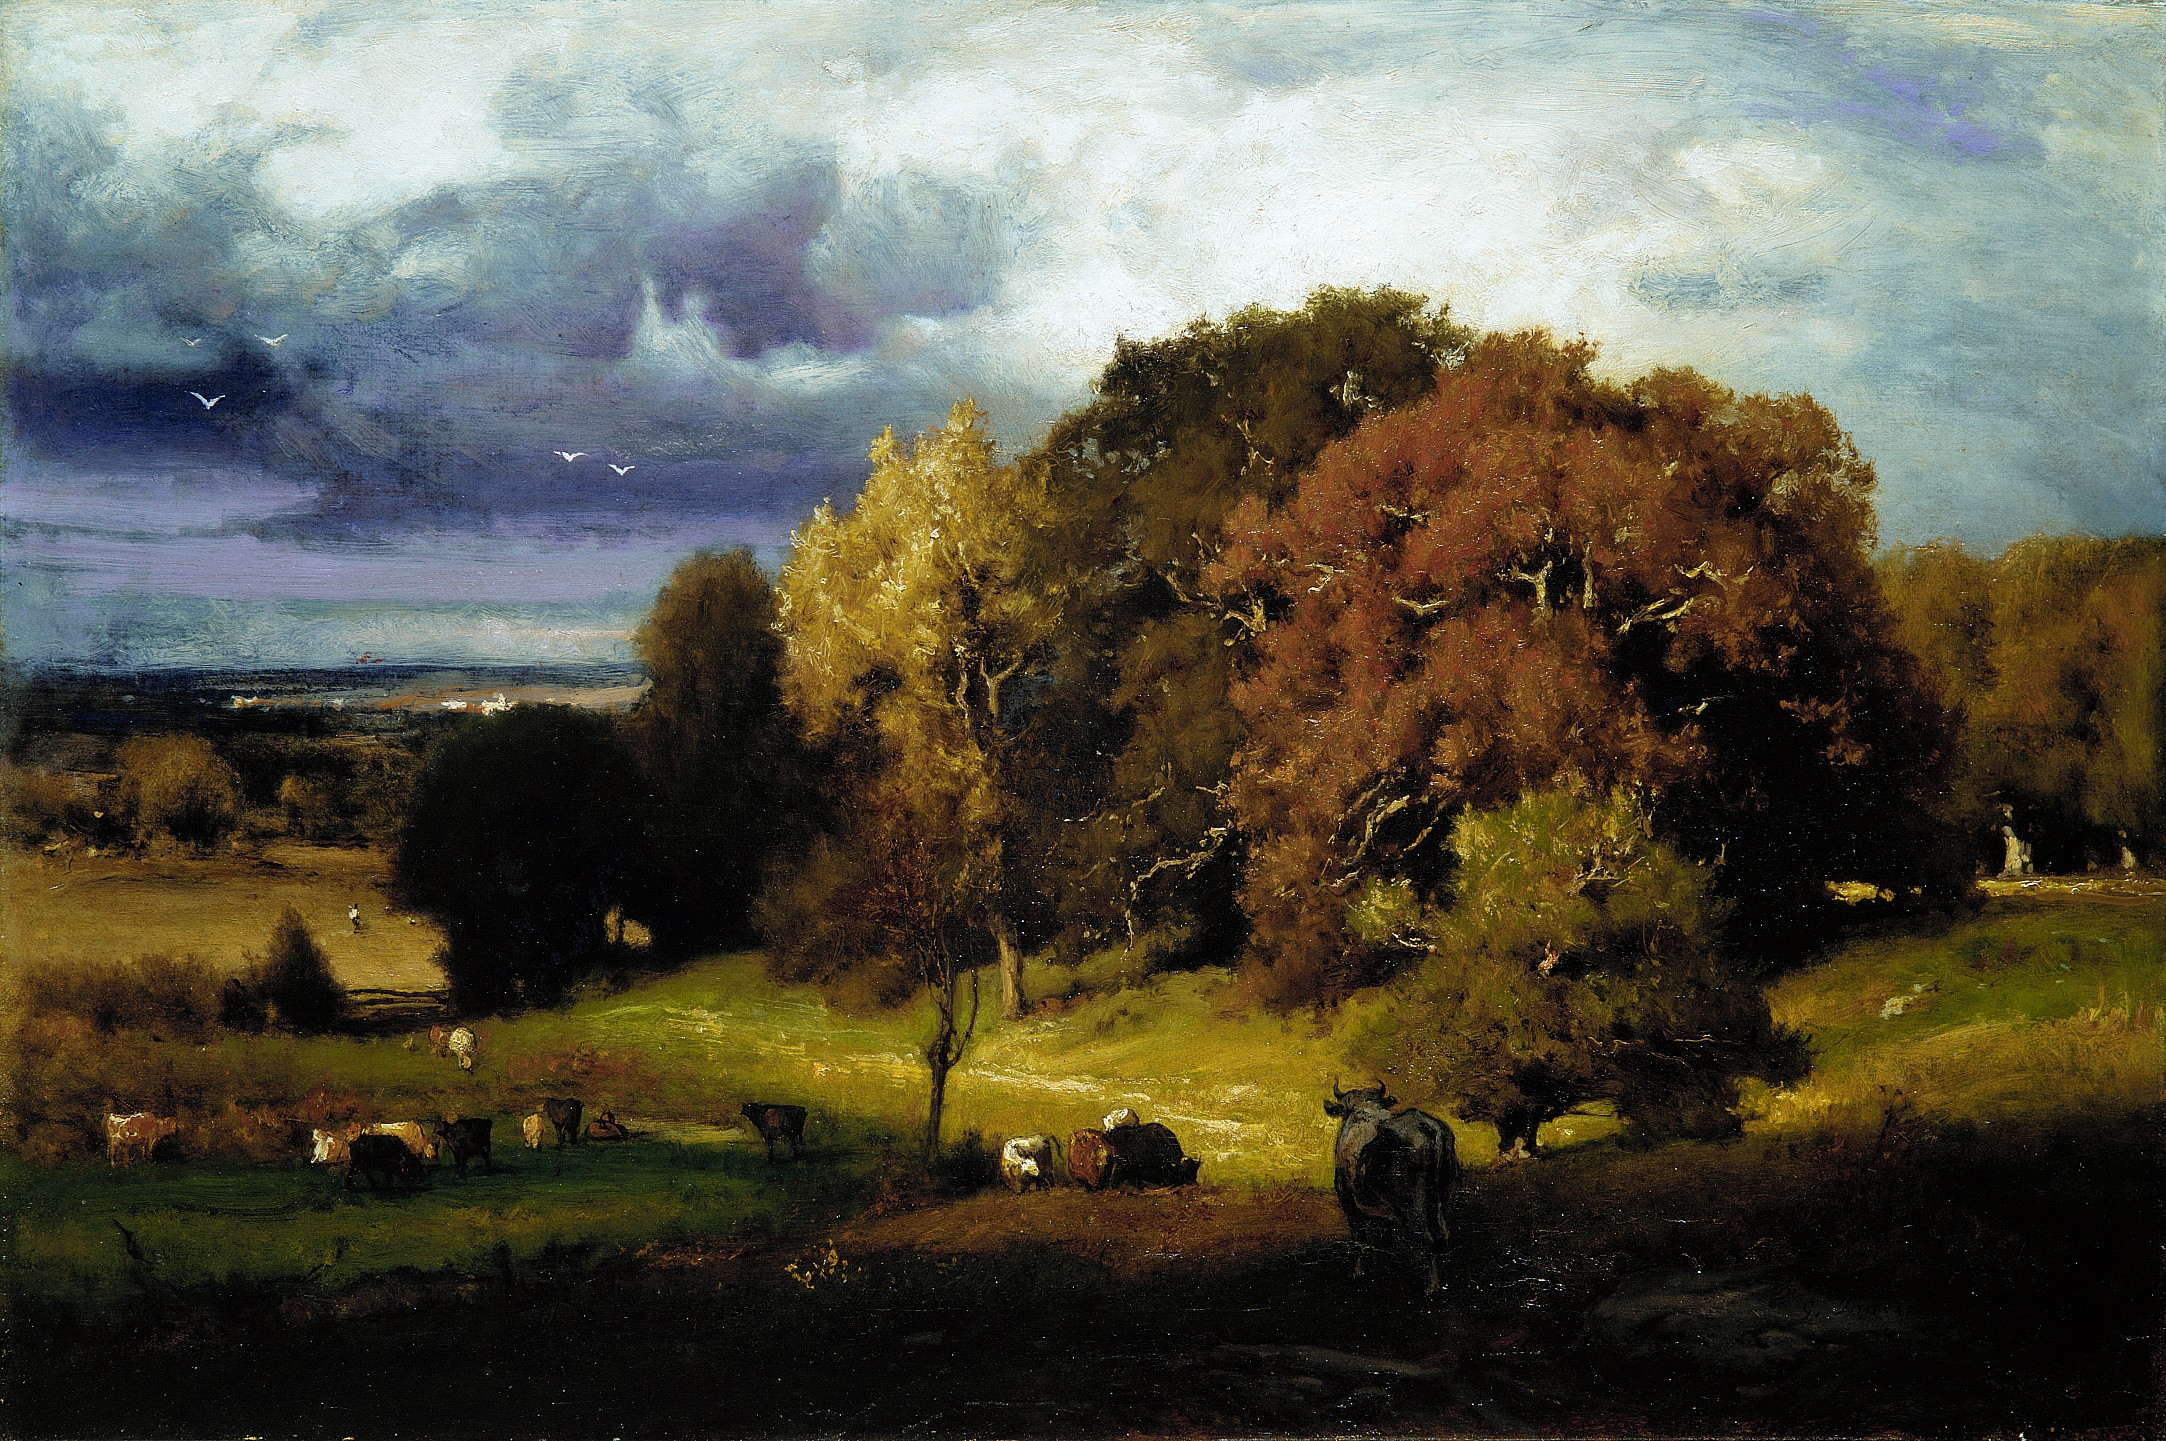
\includegraphics[width=\textwidth]{ForestPaintings/R1innessautumnoaks.jpg}
\end{minipage}
\hfill
\begin{minipage}[b]{.49\textwidth}
	\centering
	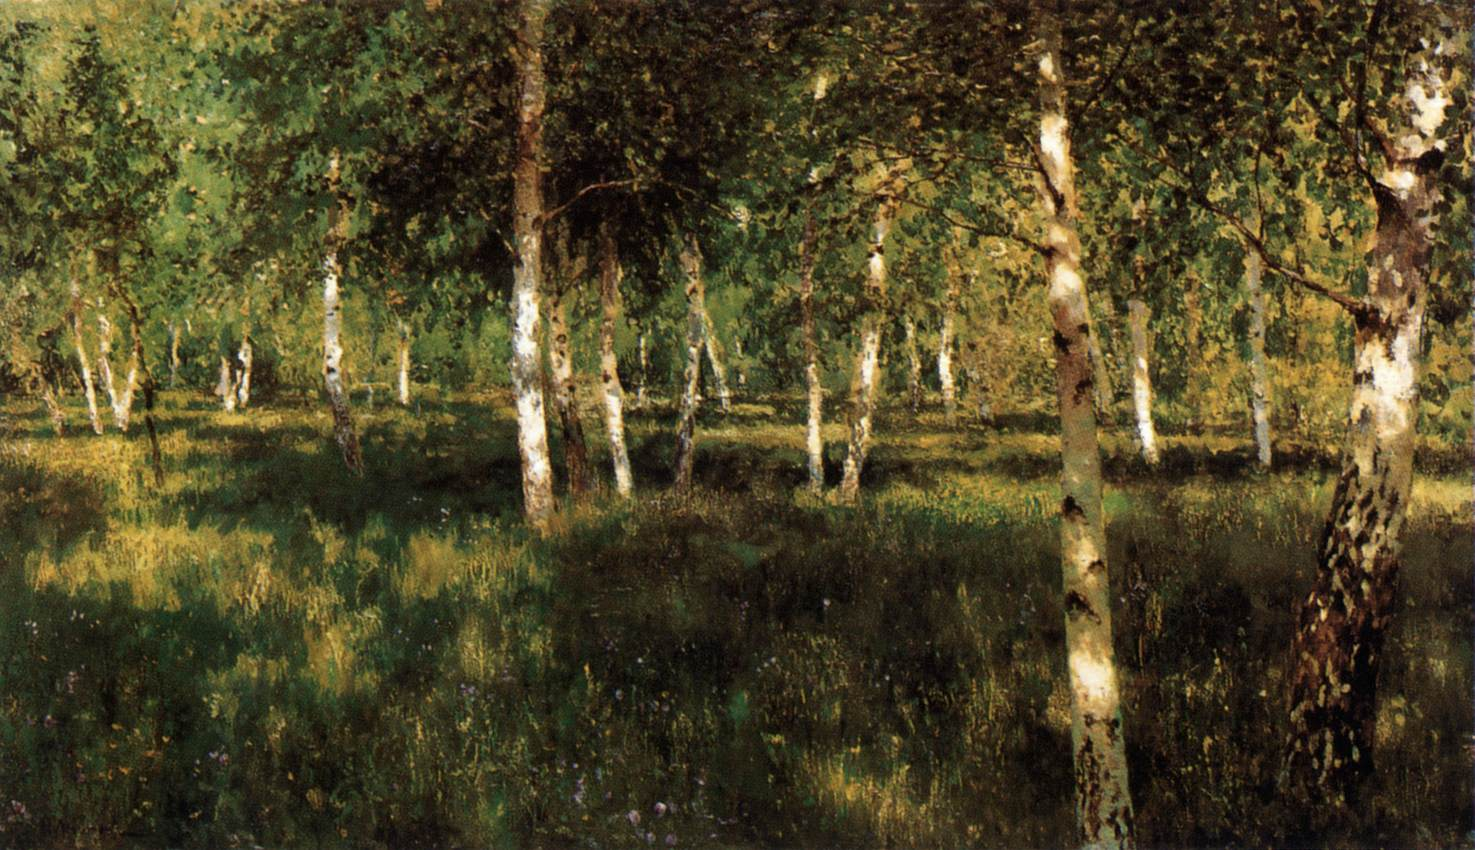
\includegraphics[width=\textwidth]{ForestPaintings/R2levitanbirchgrove.jpg}
\end{minipage}
\begin{minipage}[b]{.49\textwidth}
    \caption{\emph{Autumn Oaks} - George Inness}
\end{minipage}
\begin{minipage}[b]{.49\textwidth}
    \caption{\emph{Birch Grove} - Isaac Levitan}
\end{minipage}
\end{figure}

\subsubsection{Stylized forest paintings}
\begin {figure}[h!]
\centering
\begin{minipage}[b]{.49\textwidth}
	\centering
	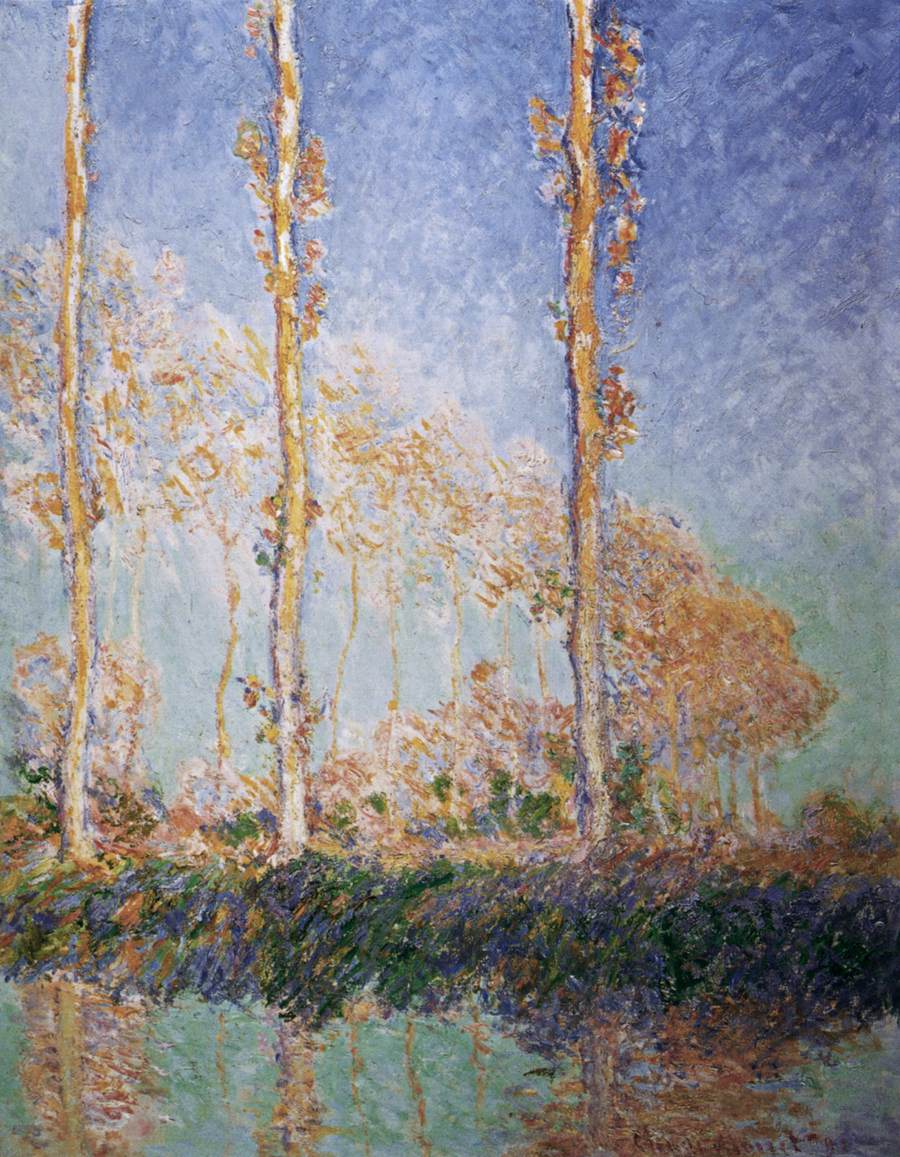
\includegraphics[width=0.9\textwidth]{ForestPaintings/S1monetpoplars.jpg}
\end{minipage}
\hfill
\begin{minipage}[b]{.49\textwidth}
	\centering
	\includegraphics[width=\textwidth]{ForestPaintings/S2hartleyautumncolor.jpg}
\end{minipage}
\begin{minipage}[t]{.49\textwidth}
	\caption{\emph{Poplars} - Claude Monet}
\end{minipage}
\begin{minipage}[t]{.49\textwidth}
	\caption{\emph{Autumn Color} - Marsden Hartley}
\end{minipage}
\end{figure}

\newpage
\subsection{Sea}

\subsubsection{Realistic seascape paintings}
\begin {figure}[h!]
\centering
\begin{minipage}[b]{.49\textwidth}
	\centering
	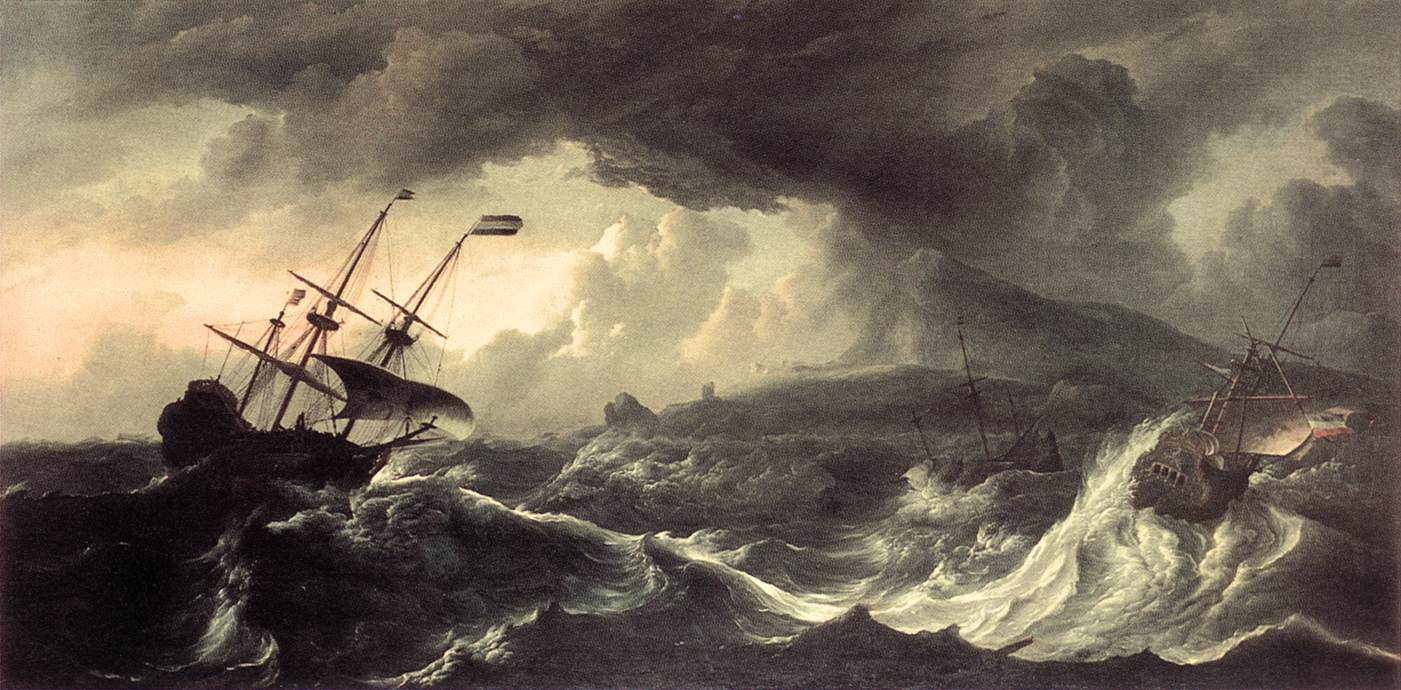
\includegraphics[width=\textwidth]{SeaPaintings/R1backhuysenshipsrunningagroundinastorm.jpg}
    \caption{\emph{Ships Running Aground in a Storm} - Ludolf Backhuysen}
\end{minipage}
\hfill
\begin{minipage}[b]{.49\textwidth}
	\centering
	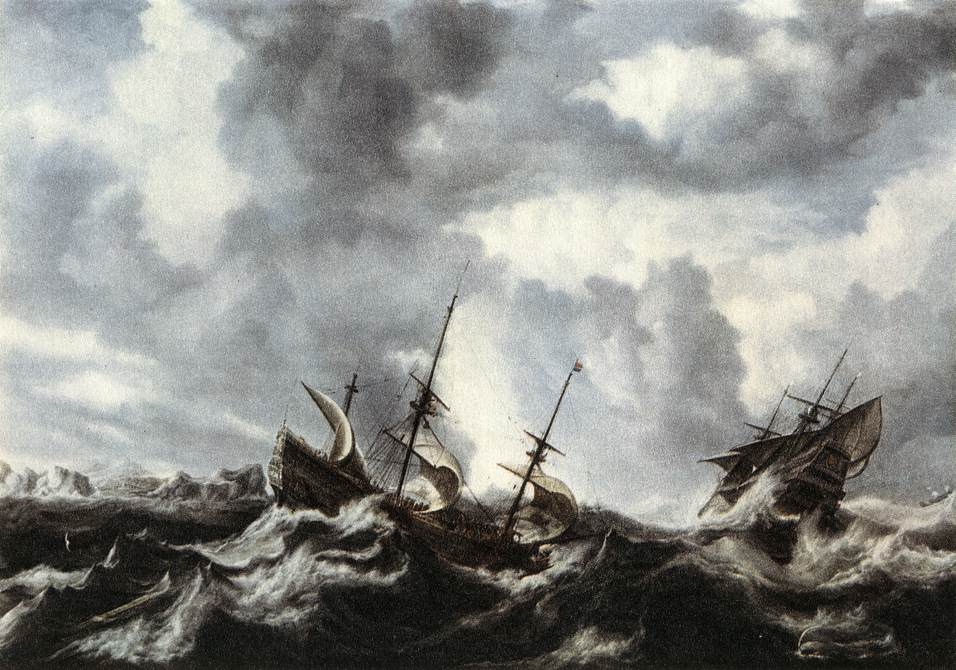
\includegraphics[width=\textwidth]{SeaPaintings/R2peetersstormonthesea.jpg}
    \caption{\emph{Storm on the Sea} - Bonaventura Peeters}
\end{minipage}
\end{figure}

\subsubsection{Stylized seascape paintings}
\begin {figure}[h!]
\centering
\begin{minipage}[b]{.49\textwidth}
	\centering
	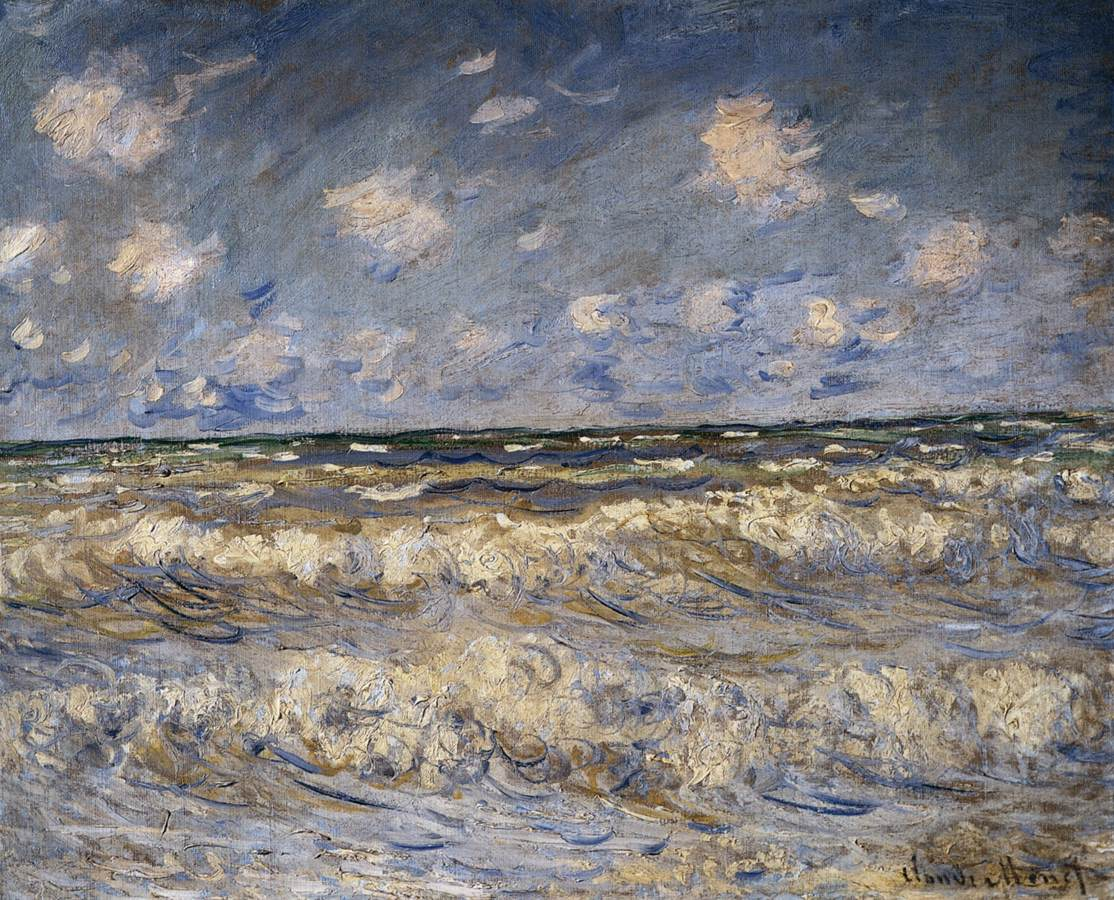
\includegraphics[width=\textwidth]{SeaPaintings/S1monetstormysea.jpg}
	\caption{\emph{Stormy Sea} - Claude Monet}
\end{minipage}
\hfill
\begin{minipage}[b]{.49\textwidth}
	\centering
	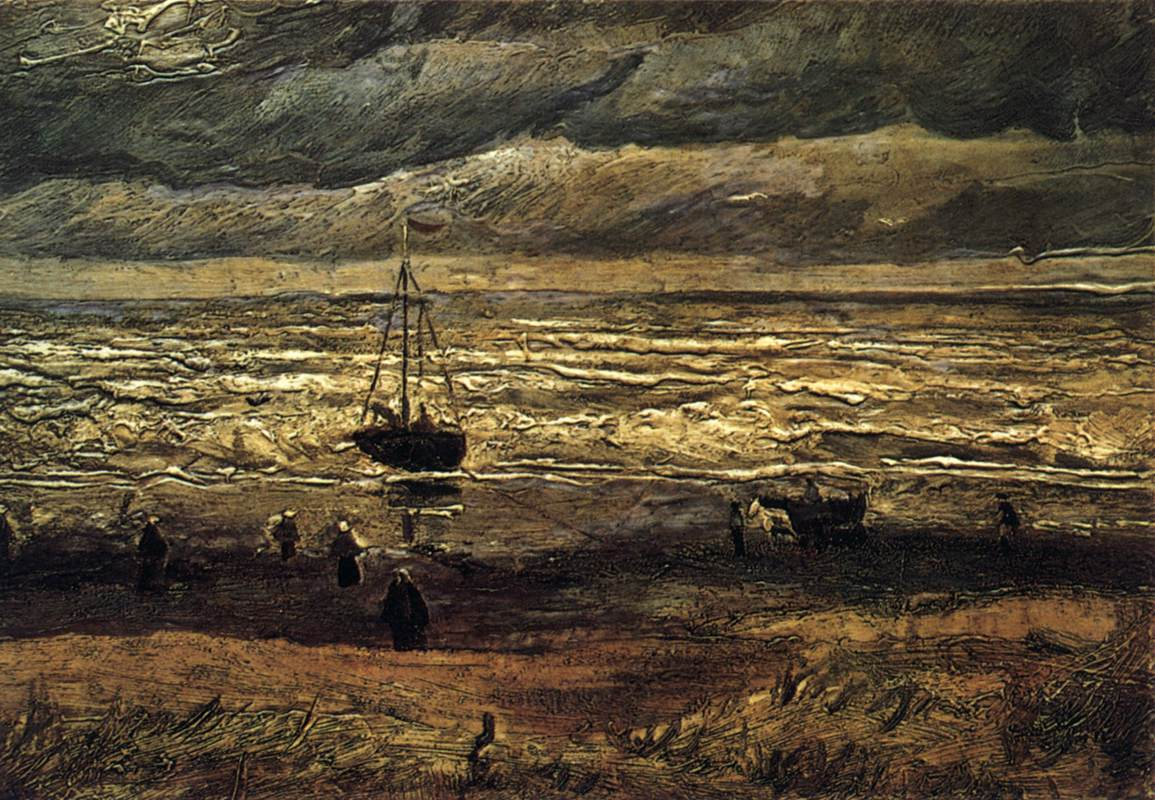
\includegraphics[width=\textwidth]{SeaPaintings/S2vangoghbeachscheveningenstormyweather.jpg}
    \caption{\emph{Beach at Scheveningen in Stormy Weather} - Vincent van Gogh}
\end{minipage}
\end{figure}

\newpage
\subsection{Snow}

\subsubsection{Realistic snow paintings}
\begin {figure}[h!]
\centering
\begin{minipage}[b]{.49\textwidth}
	\centering
	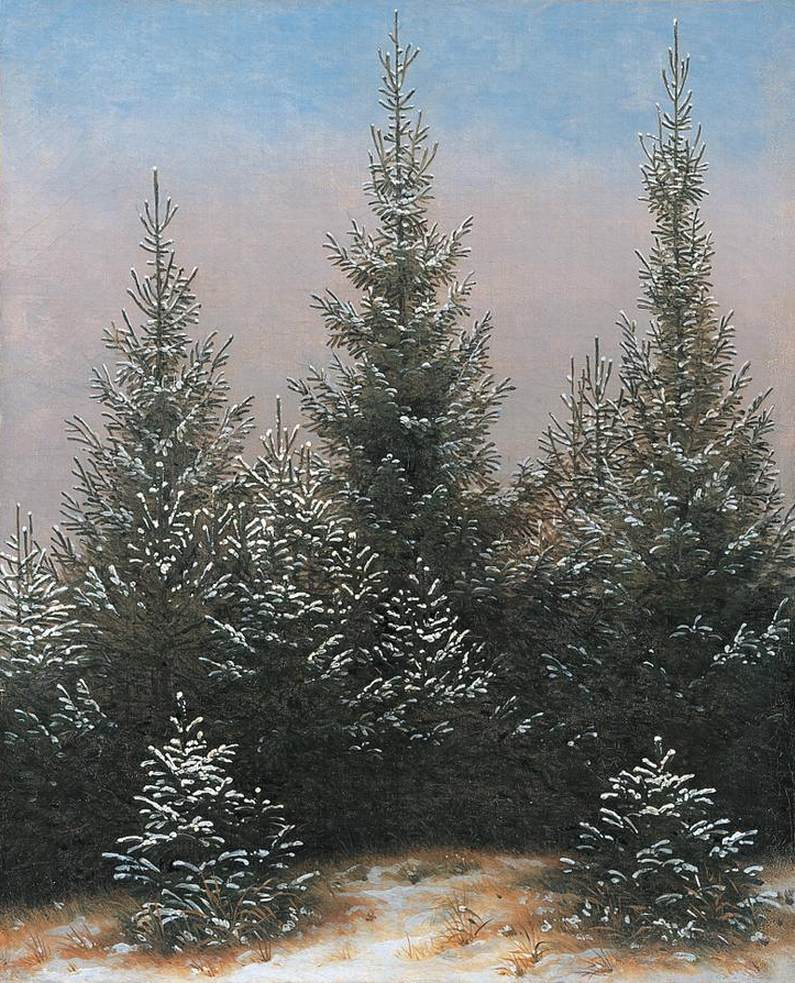
\includegraphics[width=\textwidth]{SnowPaintings/R1friedrichfirtreesinthesnow.jpg}
    \caption{\emph{Fir Trees in the Snow} - Caspar David Friedrich}
\end{minipage}
\hfill
\begin{minipage}[b]{.49\textwidth}
	\centering
	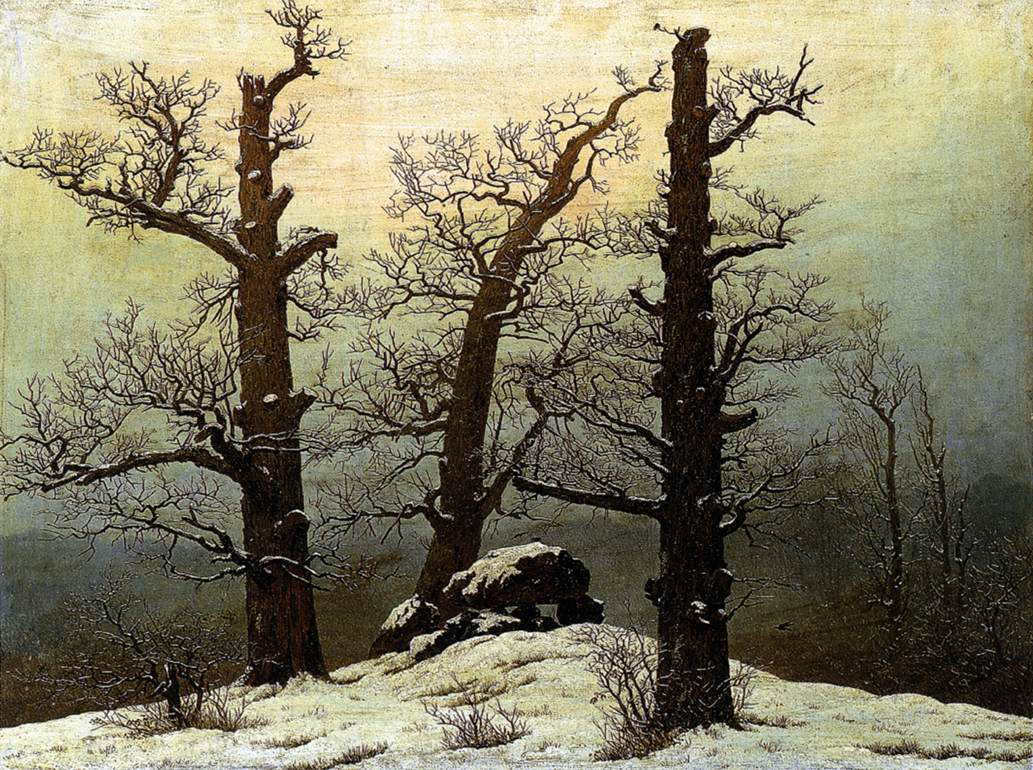
\includegraphics[width=\textwidth]{SnowPaintings/R2friedrichdolmeninthesnow.jpg}
    \caption{\emph{Dolmen in the Snow} - Caspar David Friedrich}
\end{minipage}
\end{figure}

\subsubsection{Stylized snow paintings}
\begin {figure}[h!]
\centering
\begin{minipage}[b]{.49\textwidth}
	\centering
	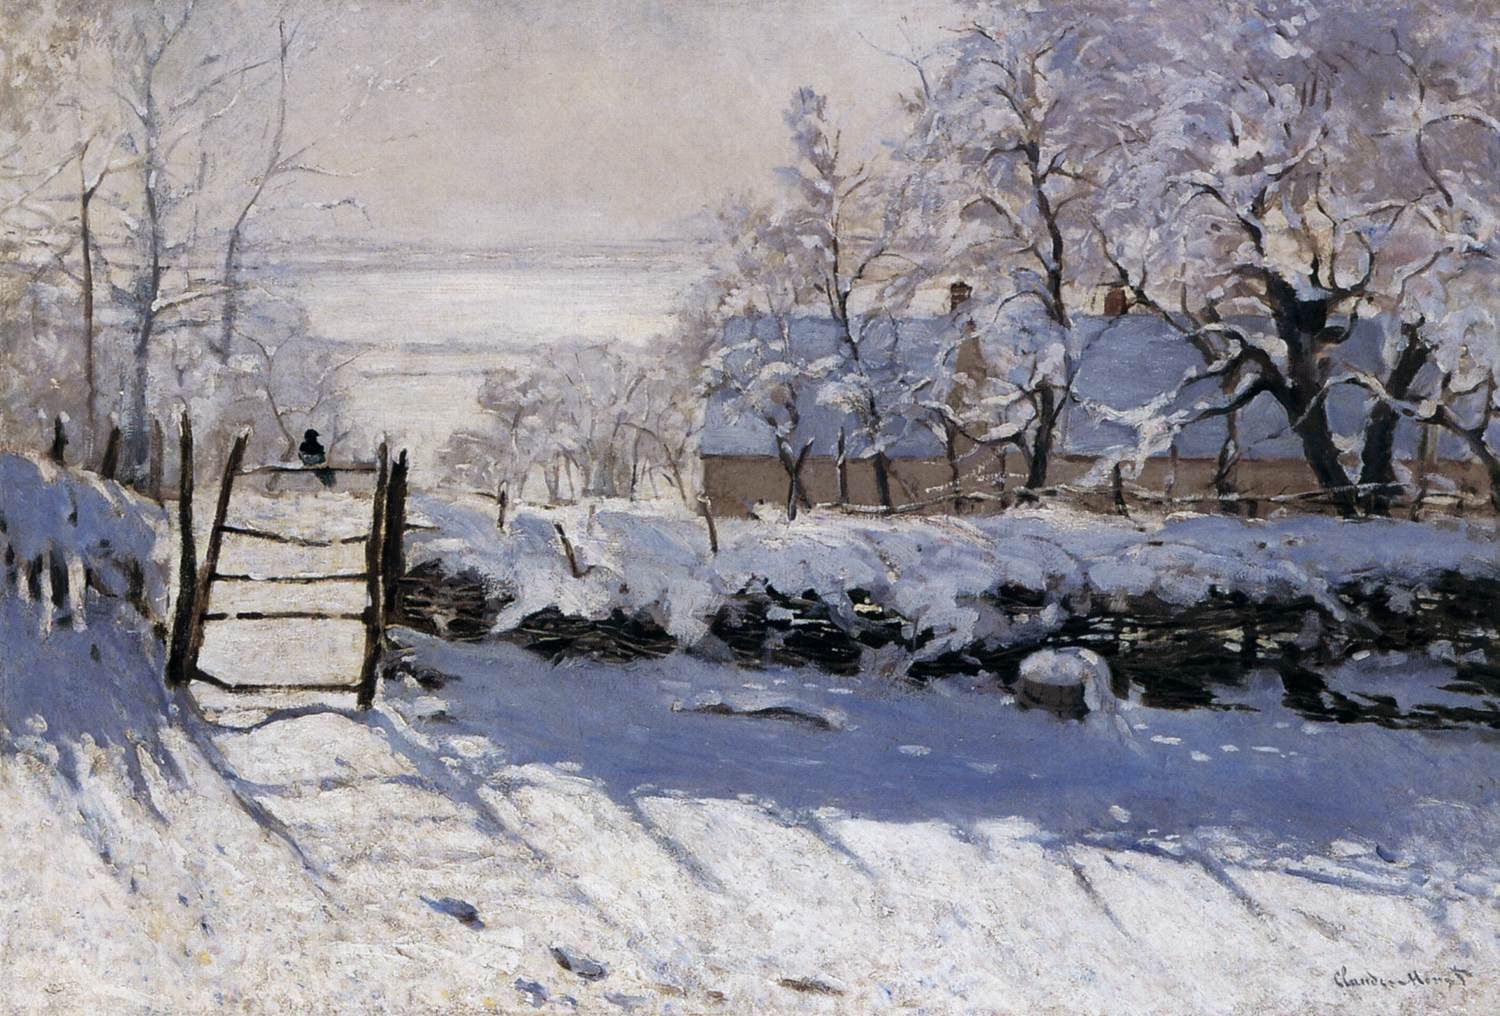
\includegraphics[width=\textwidth]{SnowPaintings/S1monetthemagpie.jpg}
    \caption{\emph{The Magpie} - Claude Monet}
\end{minipage}
\hfill
\begin{minipage}[b]{.49\textwidth}
	\centering
	\includegraphics[width=\textwidth]{SnowPaintings/S2munchtheyellowlog.jpg}
    \caption{\emph{The Yellow Log} - Edvard Munch}
\end{minipage}
\end{figure}

\end{document}